% To do: Check optimilaity claims

\documentclass{IEEEtran}

%
% If IEEEtran.cls has not been installed into the LaTeX system files,
% manually specify the path to it like:
% \documentclass[10pt,journal,compsoc]{../sty/IEEEtran}


% Some very useful LaTeX packages include:
% (uncomment the ones you want to load)


% *** MISC UTILITY PACKAGES ***
%
%\usepackage{ifpdf}
% Heiko Oberdiek's ifpdf.sty is very useful if you need conditional
% compilation based on whether the output is pdf or dvi.
% usage:
% \ifpdf
%   % pdf code
% \else
%   % dvi code
% \fi
% The latest version of ifpdf.sty can be obtained from:
% http://www.ctan.org/tex-archive/macros/latex/contrib/oberdiek/
% Also, note that IEEEtran.cls V1.7 and later provides a builtin
% \ifCLASSINFOpdf conditional that works the same way.
% When switching from latex to pdflatex and vice-versa, the compiler may
% have to be run twice to clear warning/error messages.

\usepackage{upgreek}
% *** CITATION PACKAGES ***
%
\ifCLASSOPTIONcompsoc
  % IEEE Computer Society needs nocompress option
  % requires cite.sty v4.0 or later (November 2003)
  \usepackage[nocompress]{cite}
\else
  % normal IEEE
  \usepackage{cite}
\fi


% cite.sty was written by Donald Arseneau
% V1.6 and later of IEEEtran pre-defines the format of the cite.sty package
% \cite{} output to follow that of IEEE. Loading the cite package will
% result in citation numbers being automatically sorted and properly
% "compressed/ranged". e.g., [1], [9], [2], [7], [5], [6] without using
% cite.sty will become [1], [2], [5]--[7], [9] using cite.sty. cite.sty's
% \cite will automatically add leading space, if needed. Use cite.sty's
% noadjust option (cite.sty V3.8 and later) if you want to turn this off
% such as if a citation ever needs to be enclosed in parenthesis.
% cite.sty is already installed on most LaTeX systems. Be sure and use
% version 5.0 (2009-03-20) and later if using hyperref.sty.
% The latest version can be obtained at:
% http://www.ctan.org/tex-archive/macros/latex/contrib/cite/
% The documentation is contained in the cite.sty file itself.
%
% Note that some packages require special options to format as the Computer
% Society requires. In particular, Computer Society  papers do not use
% compressed citation ranges as is done in typical IEEE papers
% (e.g., [1]-[4]). Instead, they list every citation separately in order
% (e.g., [1], [2], [3], [4]). To get the latter we need to load the cite
% package with the nocompress option which is supported by cite.sty v4.0
% and later. Note also the use of a CLASSOPTION conditional provided by
% IEEEtran.cls V1.7 and later.
% *** GRAPHICS RELATED PACKAGES ***
%
\ifCLASSINFOpdf
   \usepackage[pdftex]{graphicx}
   \usepackage{subfigure}
  % declare the path(s) where your graphic files are
  % \graphicspath{{../pdf/}{../jpeg/}}
  % and their extensions so you won't have to specify these with
  % every instance of \includegraphics
  % \DeclareGraphicsExtensions{.pdf,.jpeg,.png}
\else
  % or other class option (dvipsone, dvipdf, if not using dvips). graphicx
  % will default to the driver specified in the system graphics.cfg if no
  % driver is specified.
   \usepackage[dvips]{graphicx}
   \usepackage{subfigure}
  % declare the path(s) where your graphic files are
  % \graphicspath{{../eps/}}
  % and their extensions so you won't have to specify these with
  % every instance of \includegraphics
  % \DeclareGraphicsExtensions{.eps}
\fi


% graphicx was written by David Carlisle and Sebastian Rahtz. It is
% required if you want graphics, photos, etc. graphicx.sty is already
% installed on most LaTeX systems. The latest version and documentation
% can be obtained at: 
% http://www.ctan.org/tex-archive/macros/latex/required/graphics/
% Another good source of documentation is "Using Imported Graphics in
% LaTeX2e" by Keith Reckdahl which can be found at:
% http://www.ctan.org/tex-archive/info/epslatex/
%
% latex, and pdflatex in dvi mode, support graphics in encapsulated
% postscript (.eps) format. pdflatex in pdf mode supports graphics
% in .pdf, .jpeg, .png and .mps (metapost) formats. Users should ensure
% that all non-photo figures use a vector format (.eps, .pdf, .mps) and
% not a bitmapped formats (.jpeg, .png). IEEE frowns on bitmapped formats
% which can result in "jaggedy"/blurry rendering of lines and letters as
% well as large increases in file sizes.
%
% You can find documentation about the pdfTeX application at:
% http://www.tug.org/applications/pdftex
% *** MATH PACKAGES ***
%
\usepackage[cmex10]{amsmath}
\usepackage{amssymb}
 \usepackage{graphicx}
  \usepackage{tabulary}
  \usepackage{array,booktabs,longtable,tabularx}
% A popular package from the American Mathematical Society that provides
% many useful and powerful commands for dealing with mathematics. If using
% it, be sure to load this package with the cmex10 option to ensure that
% only type 1 fonts will utilized at all point sizes. Without this option,
% it is possible that some math symbols, particularly those within
% footnotes, will be rendered in bitmap form which will result in a
% document that cannot be IEEE Xplore compliant!
%
% Also, note that the amsmath package sets \interdisplaylinepenalty to 10000
% thus preventing page breaks from occurring within multiline equations. Use:
%\interdisplaylinepenalty=2500
% after loading amsmath to restore such page breaks as IEEEtran.cls normally
% does. amsmath.sty is already installed on most LaTeX systems. The latest
% version and documentation can be obtained at:
% http://www.ctan.org/tex-archive/macros/latex/required/amslatex/math/
% *** SPECIALIZED LIST PACKAGES ***
%
\usepackage[justification=centering]{caption}
\usepackage{url}
\usepackage{amsmath}
\usepackage{amsfonts}
\newtheorem{definition}{\noindent{\bf Definition}}
\newtheorem{lemma}{\noindent{\bf Lemma}}
\newtheorem{theorem}{\noindent{\bf Theorem}}
\newtheorem{proposition}{\noindent{\bf proposition}}



\usepackage{algorithm}
\usepackage{algorithmic}
% algorithmic.sty was written 





\begin{document}
\title{Joint source selection and transfer optimization for erasure coding storage system}
\author{\IEEEauthorblockN{Han Zhang\IEEEauthorrefmark{1}\IEEEauthorrefmark{3},  Xingang Shi\IEEEauthorrefmark{2}\IEEEauthorrefmark{3}, YingYa Guo\IEEEauthorrefmark{1}\IEEEauthorrefmark{3},Haijun Geng\IEEEauthorrefmark{4}, Zhiliang Wang\IEEEauthorrefmark{2}\IEEEauthorrefmark{3},Xia Yin\IEEEauthorrefmark{1}\IEEEauthorrefmark{3}}
\IEEEauthorblockA{\IEEEauthorrefmark{1}Department of Computer Science and Technology, Tsinghua University\\
\IEEEauthorrefmark{2}Institute for Network Sciences and Cyberspace, Tsinghua University\\
\IEEEauthorrefmark{3}Tsinghua National Laboratory for Information Science and Technology (TNLIST)\\
Beijing, P.R. China\\
\IEEEauthorrefmark{4}school  of  software  engineering, shanxi university\\
Email:\{zhanghan, wzl, yxia,guoyingya\}@csnet1.cs.tsinghua.edu.cn, \{shixg\}@cernet.edu.cn,\{genghaijun\}@sxu.edu.cn
}
}

% make the title area
\maketitle


\begin{abstract}
With the deployment of big data applications, more and more data are stored in the online storage.
Erasure coding storage system has been widely used by companies such as Google and Facebook, since it provides space-optimal data redundancy to protect against data loss. 
In erasure coding storage system, ($n$, $k$) MDS erasure code is used to divide file into $n$ chunks.
When a user want to access the file, any subset of $k$ out of $n$ chunks will be needed to reconstruct the file.
In this case, how to select $k$ out of $n$ chunks and how to let the trunks transfer quickly become important problems.
In this paper, we joint the two problems together to optimize.
Our optimization goal is to minimize average file access time (FAT).
To achieve this, we propose smallest load first heuristic to do source selection and design an online algorithm to reduce trunk transfer latency.
Base on this, we design and implement D-Target, a centralized scheduler that tries to minimize average FAT in distributed erasure coding storage system.
We then test D-Target's performance by trace-driven simulation.
Results show that, for the trace of AT$\&$T,  D-Target performs 2.5$\times$, 1.7$\times$, 1.8$\times$, 3.6$\times$ better than TCP, Aalo, Barrat and pFabric respectively.
\end{abstract}


\section{Introduction} \label{Introduction}
Social networking and e-commerce activities are popular these days and more and more data are stored in the online storage. 
Also, businesses are relying on big data analytics for business intelligence and are migrating their traditional IT infrastructure to the cloud.
In this trend, cloud storage services like Amazon's Cloud drive, Apple's iCloud, DropBox, Google Drive, Microsoft's SkyDrive, AT\&T Locker  stores redundant information on distributed servers to increase reliability for storage systems.

\begin{figure}[b]
\begin{center}
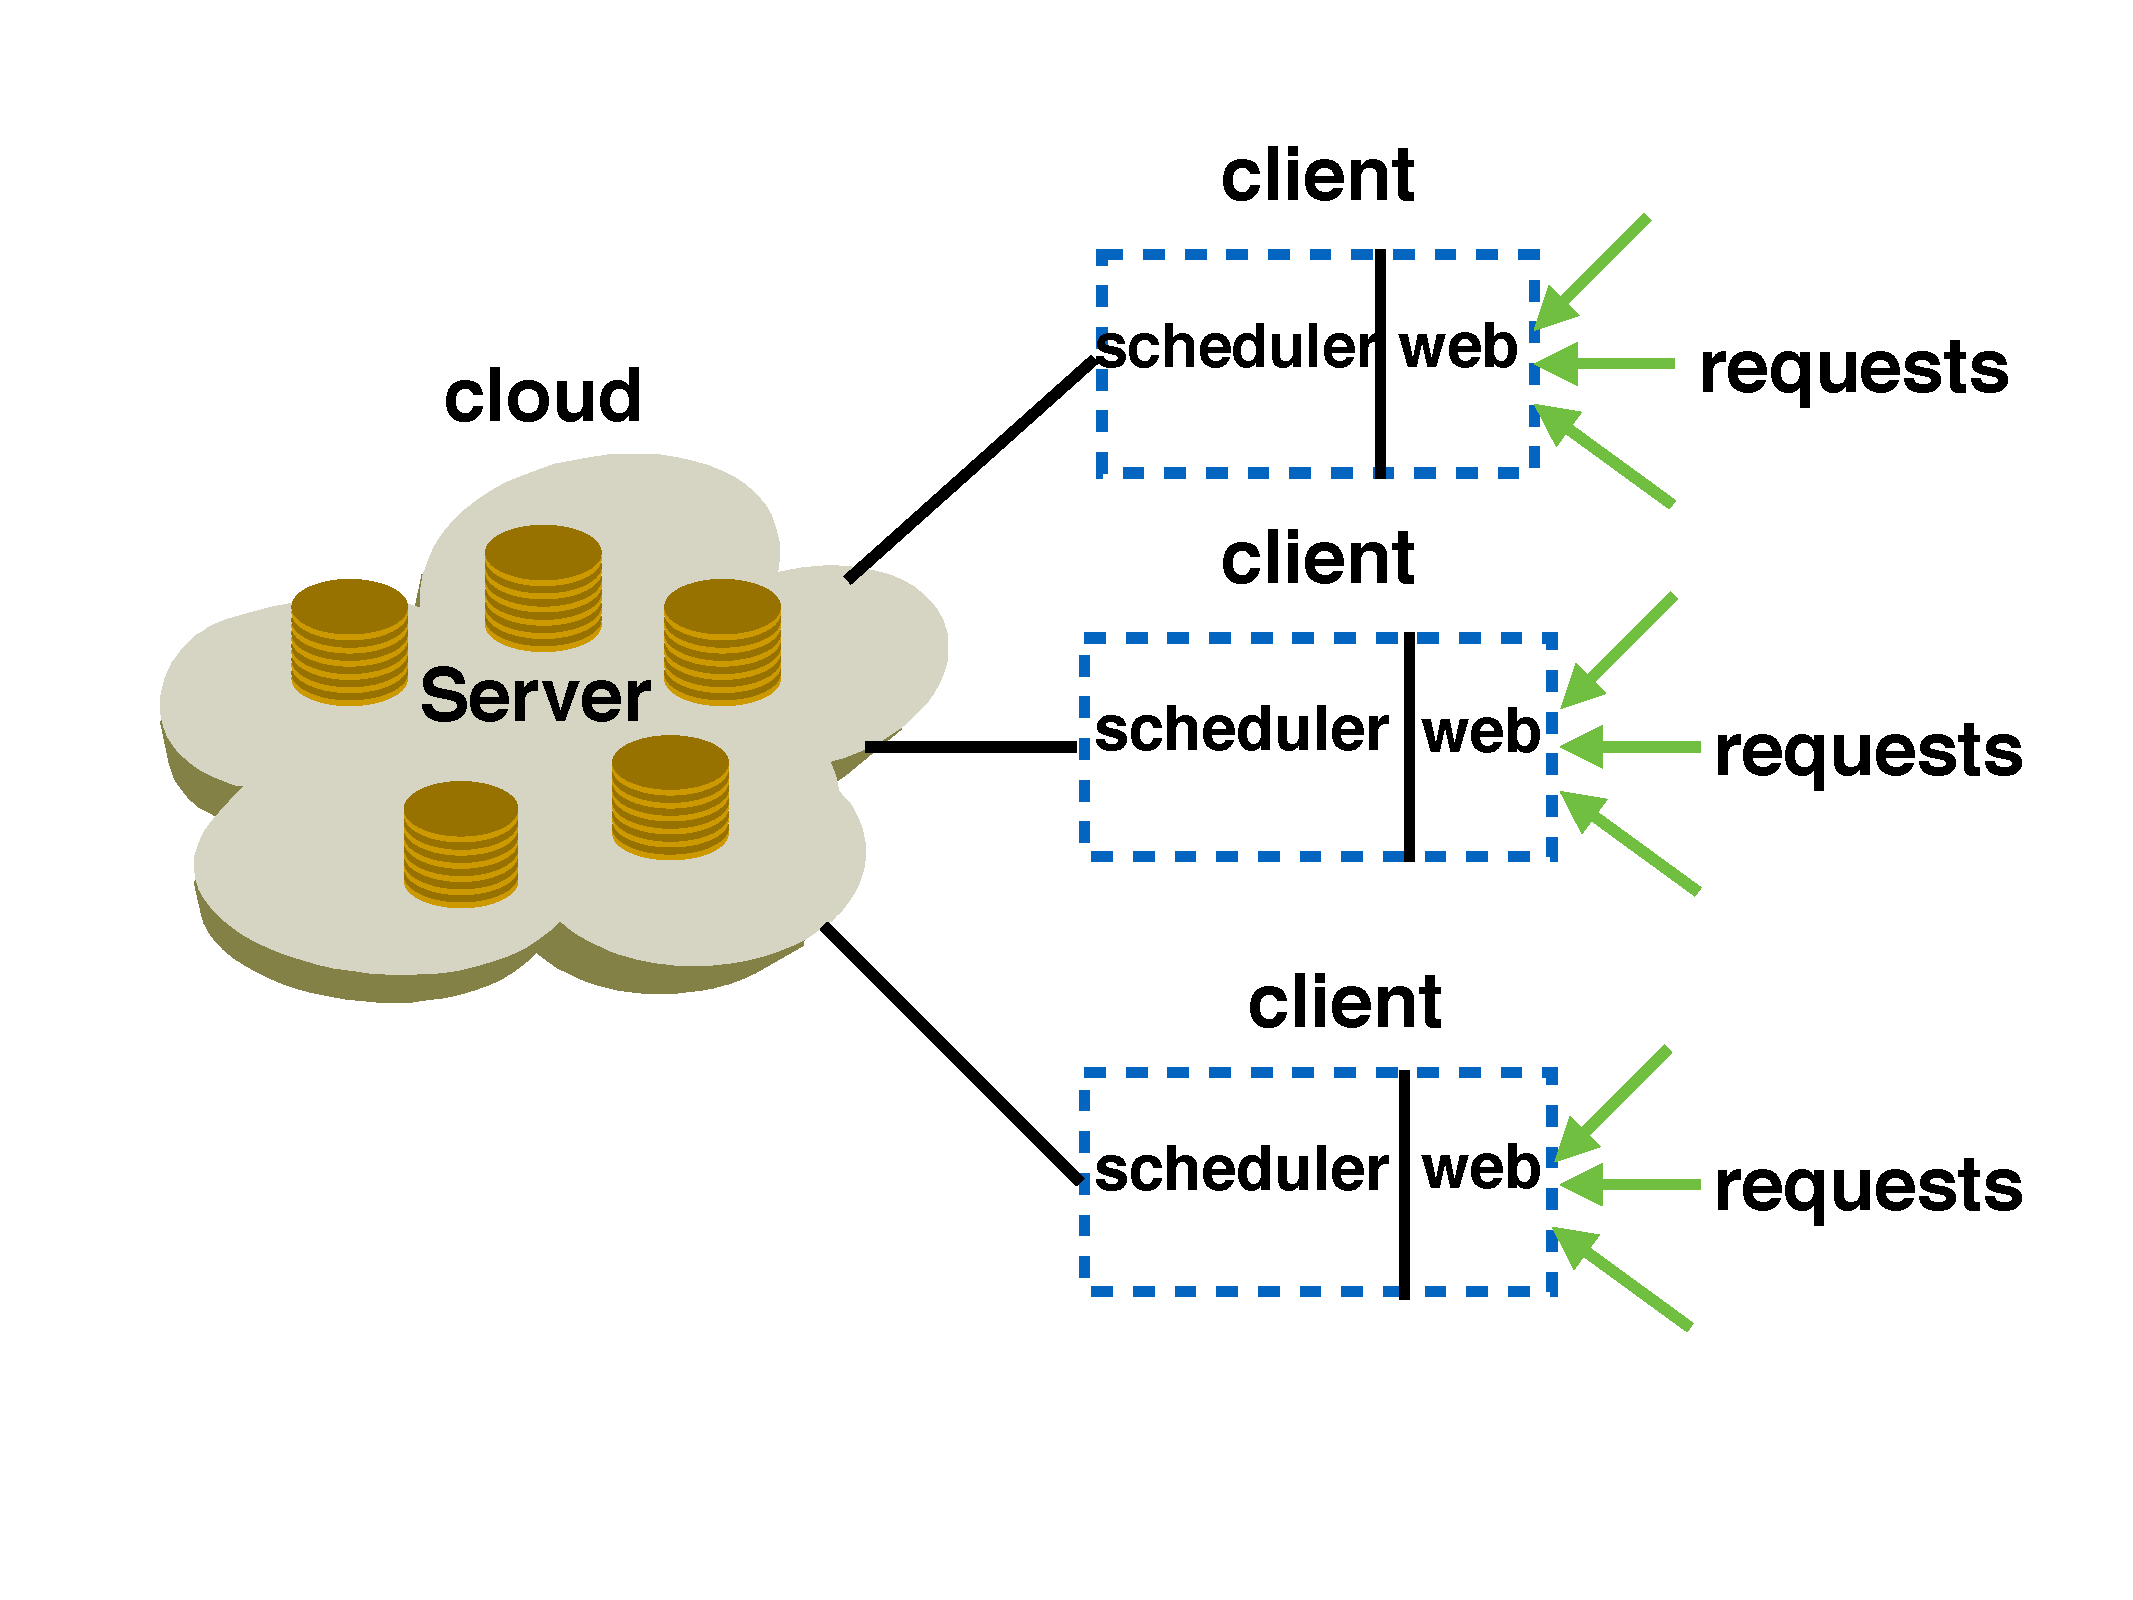
\includegraphics [width=0.7\columnwidth] {./picture/motivation/distribute.pdf}
\caption{Structure of distribute erasure coding storage system. Chunks are stored at the servers in the cloud and the clients receive requests and select sources for each request.}
\label{distribute-fig}
\end{center}
\end{figure}


Erasure coding has been widely used by companies such as Google and Facebook \cite{sathiamoorthy2013xoring} \cite{wu2010cloud}, since it provides space-optimal data redundancy to protect against data loss.
In erasure coding storage system, ($n$, $k$) MDS erasure code is used to divide file into n chunks.
When a user fetches the file, any subset of $k$ out of $n$ chunks are needed to reconstruct it. 
As Fig. \ref{distribute-fig} shown, chunks are stored at cloud servers. 
Clients receive requests from customers and the scheduler selects sources for each request. 
Then the client receives the chunks, reconstructs the file and sends the file to users.
Critical factor that affects the service quality is the delay in accessing the stored file.

We can see two processes affect the accessing latency of the distributed erasure coding storage system.
Firstly, inefficient source selection can lead to flows conflict at server nodes.
Modern distributed erasure coding storage systems always use random source selection for requests. 
This is simple, however, random source selection will make some nodes have heavy load and this will magnify latency.
To prevent this from happening, servers that have small load should be chosen to reduce the conflicts.
Secondly, tcp is not a good choice for distributed storage system.  
TCP is fair transfer method, but in erasure coding storage system, a file can be reconstructed only when the client receives all the chunks. 
For TCP transfer,  different chunks may get different bandwidth and the last finish chunk may finish late. 
This indeed wastes bandwidth as the early finish one should wait for the late ones to reconstruct the file.

In this paper, we try to minimize average file access time (FAT) for distributed erasure coding storage system.
We joint source selection and trunk transfer together to optimize.
At first, we formulate the Idealized File Access Time Minimization (IFATM) Problem.
Then we ignore the source selection and propose the Simple Idealized File Access Time Minimization (SIFATM) problem . 
We then prove even the Simple Idealized File Access Time Minimization (SIFATM) problem is NP-hard.
After this, we propose {\em smallest load first} heuristic to select sources for requests.
For the trunk transfer, we use the 2-approximate online heuristic to determine the scheduling order of trunk transfer and uses {\em Minimum-Allocation-for-Desired-Duration} (MADD) to compute the bandwidth to be allocated.
Then we evaluate D-Target, a scheduler that selects sources and allocate bandwidth for trunk transfer.
We at last use the trace of AT$\&$T to test the performance of D-Target.
Results show that D-Target performs D-Target performs 2.5$\times$, 1.7$\times$, 1.8$\times$, 3.6$\times$ better than TCP,   Aalo \cite{chowdhury2015efficient}, Barrat\cite{dogar2014decentralized} and pFabric\cite{pFabric} respectively.

Thus the contribution we make in this paper:
\begin{itemize}[\IEEEsetlabelwidth{Z}]
\item We are the first to joint source selection and trunk transfer together to optimize in distributed erasure coding storage system.
\item We formulate Idealized File Access Time Minimization (IFATM)  problem, study its hardness, and derive a non-preemptive scheduling algorithm that is 2-approximate optimal. 
\item We further design D-Target, a scheduler to select efficient sources and allocate bandwidth to trunks.
\item Trace-driven simulation shows that D-Target performs D-Target performs 2.5$\times$, 1.7$\times$, 1.8$\times$, 3.6$\times$ better than TCP,  Barrat\cite{dogar2014decentralized}, Aalo \cite{chowdhury2015efficient}, pFabric\cite{pFabric} respectively.

\end{itemize}

The rest of the paper is organized as follows. At Section \ref{motivation}, we use a small example to show the necessity of source selection and task-level transfer optimization.
Section \ref{Background} introduces the related work. 
Section \ref{sys_and_model} formulates the Idealized File Access Time Minimization (IFATM) Problem and discusses its hardness. 
Section \ref{system} presents the source selection and the design of D-Target.  
Section \ref{evaluation} evaluates D-Target against several task scheduling methods, and Section \ref{conclusion} concludes the paper.




\section{motivation} \label{motivation}

\begin{figure}[b]
\begin{center}
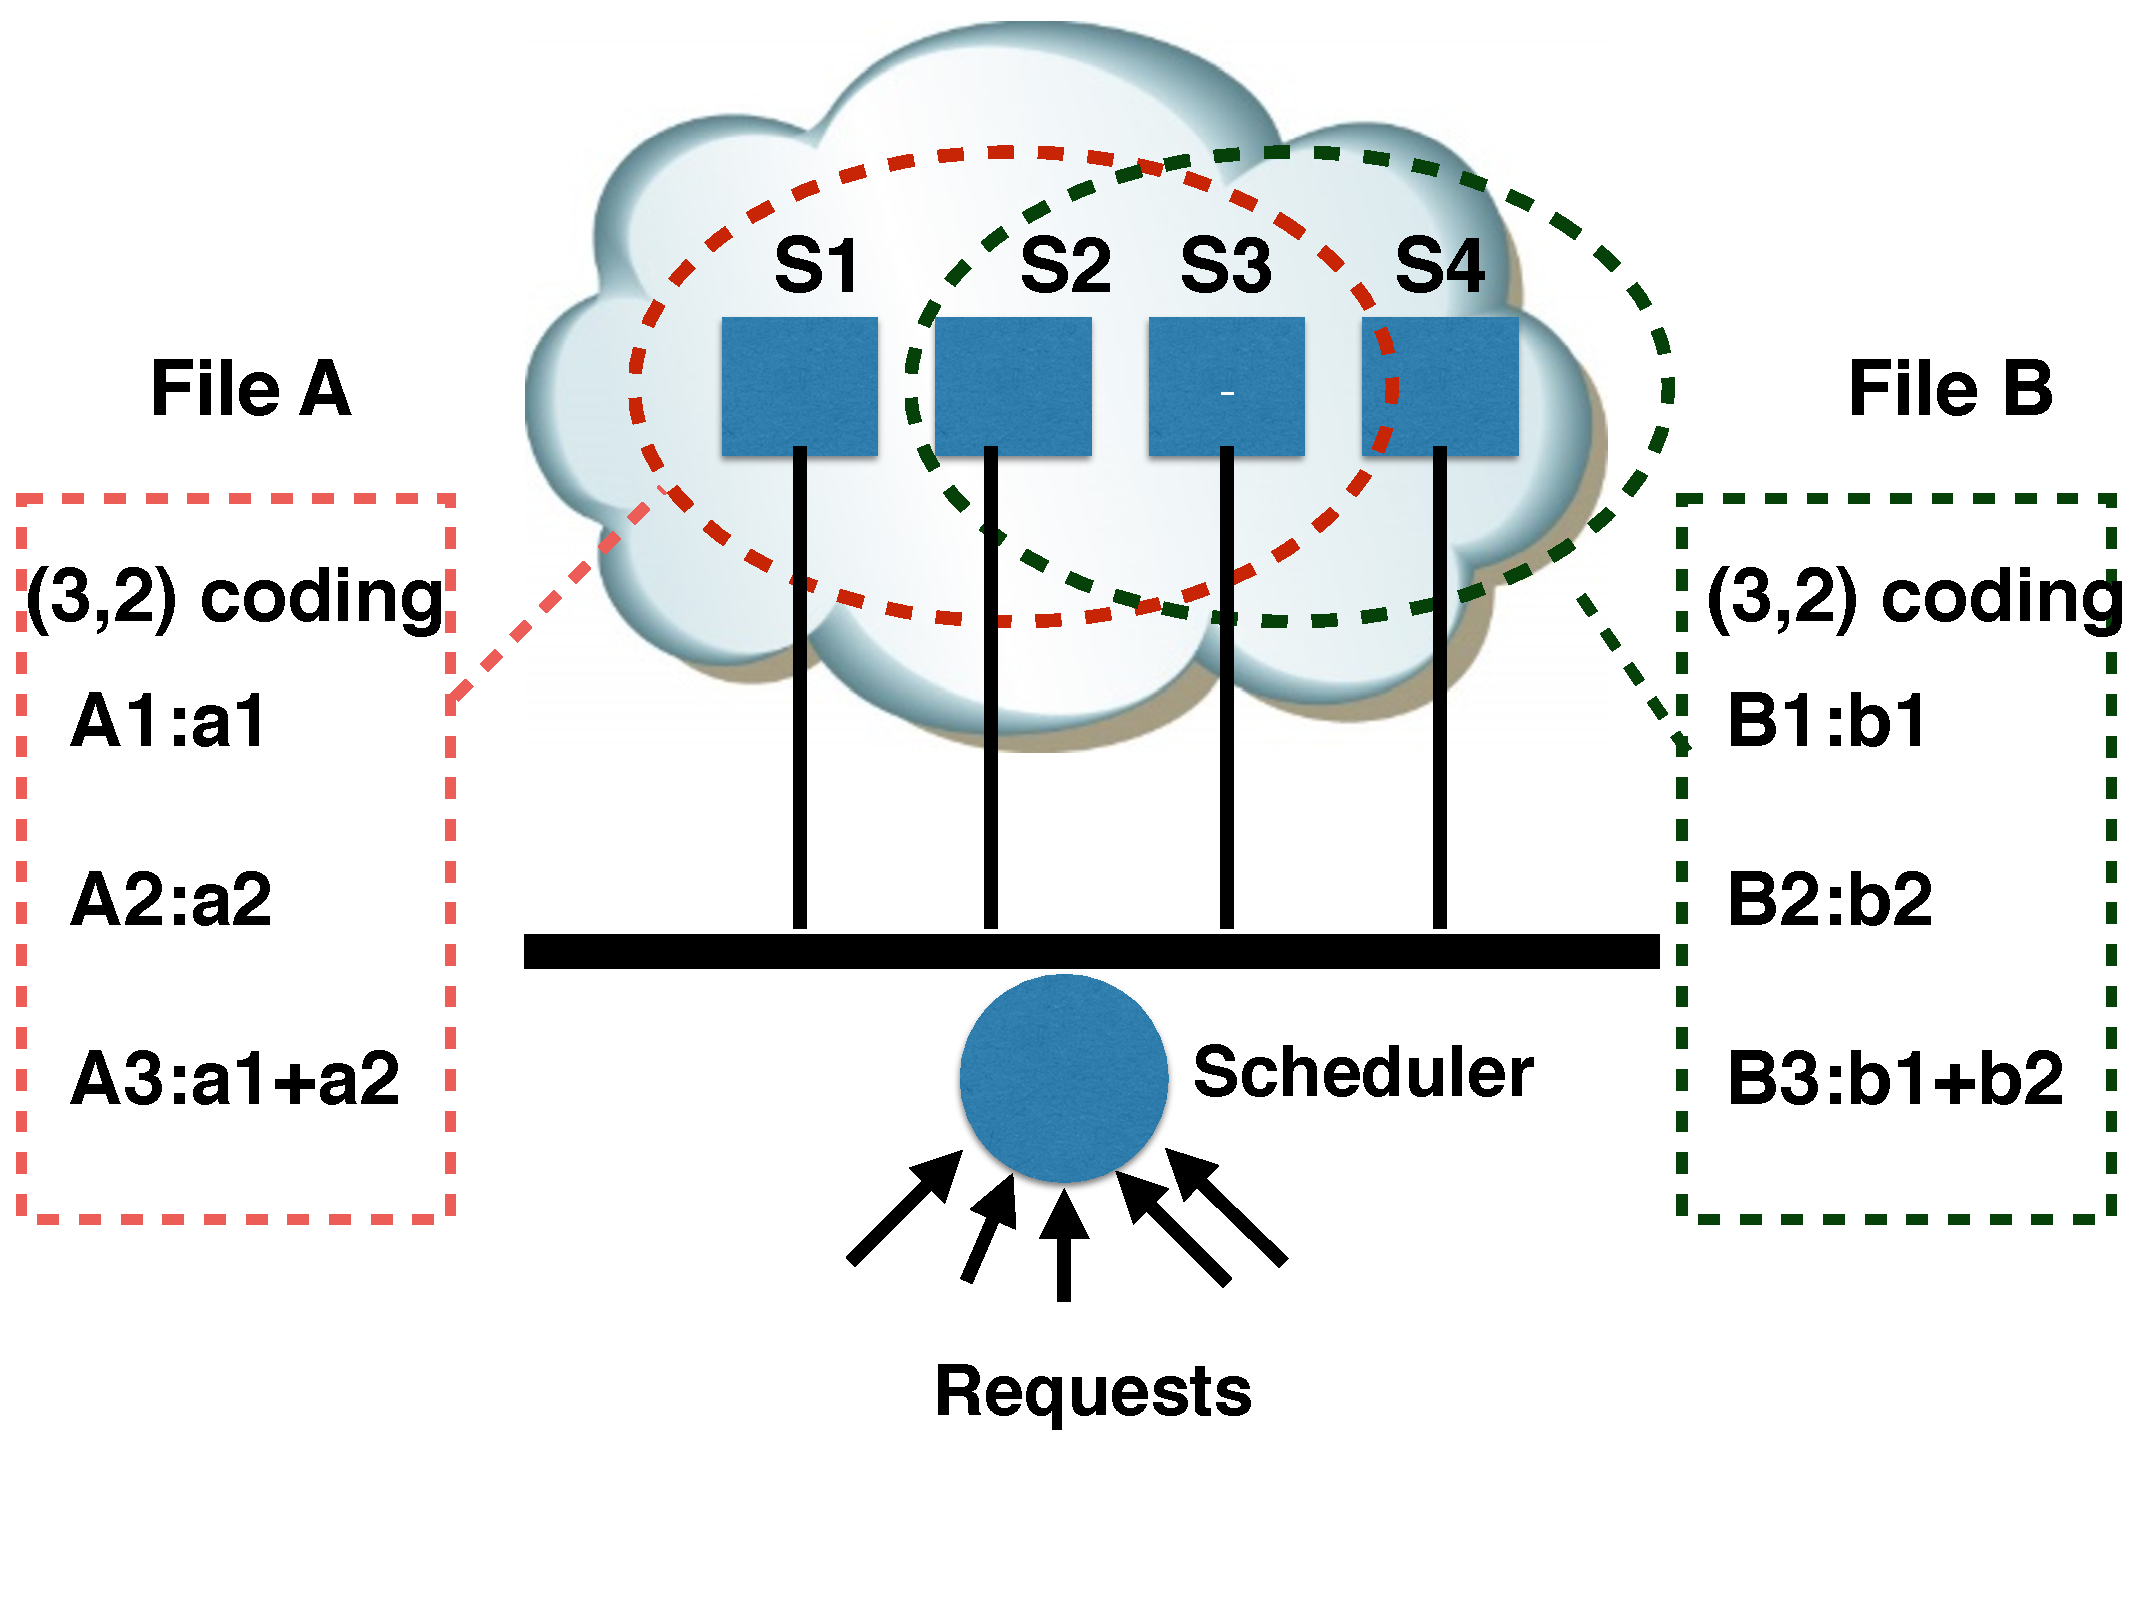
\includegraphics [width=0.7\columnwidth] {./picture/motivation/motivation.pdf}
\caption{An erasure-coding storage system contains 2 files and they are partitioned with (3, 2) MDS codes.}
\label{online-offline-fig}
\end{center}
\end{figure}

Erasure coding has been widely used by distributed storage system.
Files are encoded into chunks and chunks are stored at different machines.
When accessing a file, machine set should be chosen from the chunk nodes to reconstruct the file.
A critical factor that affects the user experiences is the delay in accessing the stored file. 
However, the bandwidth between different nodes is frequently limited and so is the bandwidth from a user to different storage nodes, which can cause significant delay in data access and perceived as poor quality of service.
In this section, we show the necessity of source selection and task-level transfer optimization for erasure coded storage system. 

In erasure coding storage system,  files are encoded into blocks using maximum distance separable (MDS) codes.
Under an $(n, k)$ MDS code, a file is encoded and stored in n storage nodes such that the chunks stored in any $k$ of these $n$ nodes suffice to recover the entire file. 
As Fig. \ref{online-offline-fig} shown, we consider two files A and B, both encoded and stored at $n=3$ machines.
A request to retrieve file A can be completed after it is successfully processed by $2$ distinct nodes chosen from $\{S1,S2,S3\}$.
It is similar for file B, which can be chosen from $ \{S2,S3,S4\}$.
To simplify the problem, we assume capacity of all links is 1 and chunk size of file A and file B is also $1$.
Firstly, we consider two requests $R_{A}$ and $R_{B}$ that arrive simultaneously at $ t =0$ to fetch file A and file B respectively.
For $R_{A}$, file A has $3$ source selection options: $(S1,S2), (S1,S3), (S2,S3)$, while file B has $(S2,S3), (S2,S4), (S3,S4)$.
If the scheduler uses random source selection, a common case maybe $R_{A}$ chooses $(S2,S3)$ and $R_{B}$ chooses $(S3,S4)$.
If the transfer policy is TCP, then the file access time for $R_{A}$ is $t_{A}=2$ and for  $R_{B}$ is $t_{B}=2$.
The AFAT(average file access time) is $2$.
However, if $R_{A}$ chooses $(S1,S2$) and $R_{B}$ chooses $(S3,S4)$, the AFAT is $1$. 
From the simple example, we can see, for the erasure coding storage system, 
efficient source selection for request can reduce AFAT, thus user experience will be better.

What's more, only tcp-fair transfer is not enough for the distributed storage system.
Just think the simple case, there are two request for file A, $R_{A_1}$ arrives at $t=0$ and $R_{A_2}$ arrives at $t=0.1$.
$R_{A_1}$ chooses$ (S1,S2)$ as the sources and $R_{A_2}$ chooses $(S2,S3)$ as the sources.
For TCP transfer, FAT( file access time) for $R_{A_1}$ is $t=1.9$ and FAT for $R_{A_2}$ is $t=2.0$,
so that AFAT( average file access time)  is $(1.9+2.0)/2=1.95$.
However, if we let $R_{A_1}$  have higher priority than  $R_{A_2}$.
Then FAT for $R_{A_1}$ is $t=1$ and FAT for $R_{A_2}$ is $t=2$,
so that AFAT is $(1+2)/2=1.5$. 
We can see, incorporating task level optimization can improve much on reducing AFAT for file transfer in distributed storage system.

From the two simple examples, we can see that both source selection and file transfer optimization play important roles
in reducing FAT(file access time).
In this paper, we join the two problems together to optimize.



\section{Background and related work} \label{Background}

It has been reported that the storage space used for photo storage only in Facebook 
has been over 20 PB in 2011 and is increasing by 60 TB every week \cite{beaver2010finding} \cite{li2013erasure}.
As massive data stores on disk, there can be a large number of failures everyday.
To compensate for the data loss and thus to guarantee the integrity of data stored in the cloud, 
it is natural to store replicas in multiple disks, such that data losses can be tolerated as long as there is at least one replica available\cite{li2013erasure}.
However, just storing the reputation of data can reduce the efficiency of storage space.
Erasure coding is used to encode data into a set of trunks and a file can be reconstructed by a subset of total trunks.
This method can compensate for the data loss and thus to guarantee the integrity of data stored in the cloud.

Although erasure coding storage system can guarantee the integrity of data, however,
as reading or writing data, the system needs to encode or decode data,
 leading to a high access latency and a low access throughput due to the CPU limit,
 so that previous work  \cite{lin2012secure},\cite{dimakis2010network},\cite{dimakis2006decentralized},\cite{dimakis606049decentralized} mainly focus on
 efficient encoding and decoding.
 By efficient encoding technology,  overhead of CPU will significantly reduce.
 However, though erasure coding stores data as multiple coded blocks, 
 when accessing file or one coded block getting lost, 
 the system must get multiple coded blocks that are sufficient to recover all the data.
 This process can add large burden to network.
Indeed, latency optimization has attracted more and more attention, even Google and Amazon have published that every additional 500ms can
lead to 1.2\% user loss \cite{schurman2009user}. 
Optimizing the transfer latency of shares is very important, as this can improve user experience, thus revenue.
Still now, lots of methods have been proposed to reduce applications' transfer latency in data center.
According to schedule granularity, we can divide them into two kinds: flow level optimization and task level optimization.

DCTCP \cite{DCTCP}, D$^2$TCP \cite{D2TCP}, L$^2$DCT \cite{L2DCT}, PDQ \cite{PDQ}, pFabric\cite{pFabric}, LPD\cite{zhang2015more},
D$^3$\cite{D3} are flow level methods.
DCTCP is fair sharing method and it tries to maintain the switch's queue shallow to reduce queue delay.
However, in data center, applications have different demands of bandwidth and fair sharing is not a good choice \cite{zhang2016fdrc}.
D$^2$TCP, LPD, D$^3$ are deadline-aware bandwidth allocation methods.
They set explicit deadline to flows which have different emergency, so that tight flows will get more bandwidth than the lax ones.
As a result, applications' demand will be satisfied.
L$^2$DCT, PDQ, pFabric try to minimize average flow completion time.
They assume short flows are always the emergency ones which need to finish transfer as fast as possible. 
They throttle the bandwidth of large flows and spare the bandwidth to the short ones. 
Then the short flows transfer faster than the large ones. 
As a result, average flow completion time reduces. 
Although flow-level optimization methods perform better than TCP on latency optimization,
however, in data center network, distributed applications always have parallel flows and just flow-level
optimization is not enough.
Task-level schedule methods such as Barrat\cite{dogar2014decentralized}, Varys\cite{chowdhury2014efficient}, Aalo \cite{chowdhury2015efficient}, sunflow\cite{huang2016sunflow} regard flows of applications as a whole.
Barrat  \cite{dogar2014decentralized} schedules tasks in FIFO order but avoids head-of-line blocking by dynamically changing the level of multiplexing in the network. 
Varys\cite{chowdhury2014efficient} regards applications'  parallel flows as coflow and it uses SEBF to schedule coflows and MADD to perform rate control, as a result, average task completion time will reduce.
Aalo \cite{chowdhury2015efficient} ,sunflows \cite{huang2016sunflow}, and CODA \cite{zhang2016coda} do not need to know coflow information beforehand. 
In erasure coding storage system, file access will generate parallel flows. We think just flow level optimization is not enough,
task level schedule methods should be considered to make the transfer efficiency.




%\begin{figure*}[!htb]
%\centering
%\subfloat[percentage of flows missing deadline]{
%\label{spine-dc-data2-1}
%\includegraphics[width=0.25\textwidth]{picture/motivation/motivation_schedule}}
%\subfloat[average flow completion time]{
%\label{spine-dc-data2-5}
%\includegraphics[width=0.25\textwidth]{picture/motivation/motivation_varys}}
%\subfloat[background traffic bandwidth]{
%\label{spine-dc-data2-30}
%\includegraphics[width=0.25\textwidth]{picture/motivation/motivation_optimal}}
%\subfloat[background traffic bandwidth]{
%\label{spine-dc-data2-30}
%\includegraphics[width=0.25\textwidth]{picture/motivation/motivation_routing}}
%\caption{motivation example: 50\% of flows have explicit deadline while the other flows should transfer as quickly as possible }
%\label{motivation-fig}
%\end{figure*}

\section{Network model and Analysis} \label{sys_and_model}

In this section, we first introduce the data center non-blocking model, and then propose Idealized File Access Time Minimization (IFATM) Problem.
At last, we simplify the problem and prove even the simplified IFATM problem is NP-hard.


\subsection{Network model}
Recent studies \cite{pFabric},\cite{chowdhury2014efficient},\cite{huang2016sunflow},\cite{chowdhury2015efficient},
regard the data center as a big switch, where all ports have normalized united capacity.
All flows compete for the ingress and egress bandwidth.
Such  abstraction is reasonable and matches with recent full bisection bandwidth topologies widely used in current production data centers \cite{luo2016towards}.
In this paper, we use this assumption and only take the contention of ingress and egress ports into consideration.

\subsection{Problem formulation}
We consider a non-blocking data center that consists of $n$  storage nodes, denoted by $\mathcal{S} = \{s_1,s_2,...s_n\}$.
Then $r$ files, denoted by $\mathcal{F}=\{f_1,f_2,f_3..f_r\}$ are stored in the server set.
For each file $f_i$, we partition it into $k_i$ fixed-size trunks and then encode it 
using an $(n_i,k_i)$ MDS erasure code to generate $n_i $ distinct trunks of the same size for $f_i$.
The $n_i$ distinct shares are stored at $n_i$ machines.
The use of $(n_i, k_i)$ MDS erasure code allows the file to be reconstructed from any subset of $k_i$-out-of-$n_i$ trunks, 
whereas it also introduces a redundancy factor of $n_i / k_i$.
The m clients, denoted by $\mathcal{C}=\{c_1,c_2...c_m\}$.
Assume all the $L$ requests arrive at time 0 and the $k-th$ request denoted by $T^{(k)}_{f^k}$ means requesting file $f^k(f^k\in \mathcal{F})$.
The k-th request $T^{(k)}_{f^k} $consists of parallel subtasks, each subtask is a flow from a server to the client.
$T^{(k)}_{f^k}=\{t_{i,j}^{(k,f^k)}|1 \le i \le n ,1\le j \le m\}$, where $t_{i,j}^{(k,f^k)}$ presents a sub-task whose size is $t_{i,j}^{(k,f^k)}$.
$x^{(k,f^k)}_{i,j}  \in \{0,1\}$ , where 1 denotes that there is a flow from server i to client j and 0 denotes there is no flow  from server i to client j.
As the non-blocking model's ingress and egress ports have unit capacity,
so the transfer time for sub-task $t_{i,j}^{(k,f^k)}$ is  $t_{i,j}^{(k,f^k)}$.
The problem of non-preemptive Idealized File Access Time Minimization (IFATM) Problem can be defined as:
 \begin{eqnarray}
&\d {\rm minimize} & \sum_{g=1}^{L} C_{g} \label{eq:ECSF-SC} \\
& \d{\rm s.t.} &\forall g,j\sum_{\forall l:C_l \leq C_g}\sum_{i=1}^{n}t_{i,j}^{(l,f^l)}*x_{i,j}^{(l,f^l)}\leq C_g  \label{eq:ingress_constraint}\\
&&\forall g,i\sum_{\forall l:C_l \leq C_g}\sum_{j=1}^{m}t_{i,j}^{(l,f^l)}*x_{i,j} ^{(l,f^l)} \leq C_g   \label{eq:egress_constraint}\\
&& \forall l,j\sum_{i=1}^nx_{i,j}^{(l,f^l)}=k_{f^l}  \label{eq:source_constraint}
\end{eqnarray}

Our goal is to minimize the average file access time. 
The constraints (\ref{eq:ingress_constraint}) and (\ref{eq:egress_constraint}) are due to the competition on the capacity of each port. 
For a request $T^{(k)}_{f^k}$ with completion time $C_{k}$ , consider the set of file transfer that finish before it, i.e., $T^{(l)}_{f^l}$: $C_{l} \le C_{k}$. For any ingress port i (or egress port j), the file access time on this port is at least  $\sum_{\forall l:C_l \leq C_g}\sum_{i=1}^{n}t_{i,j}^{(l,f^l)}*x_{i,j}^{(l,f^l)}$(or  $\sum_{\forall l:C_l \leq C_g}\sum_{j=1}^{m}t_{i,j}^{(l,f^l)}*x_{i,j} ^{(l,f^l)}$ , correspondingly), which must no longer than $C_{k}$.
(\ref{eq:source_constraint}) describes source selection, which means that the scheduler should selects $k_{f^l}$ servers for file ${f^l}$. 


\subsection{NP-hard proof}
In this part, we prove  Idealized File Access Time Minimization (IFATM) problem is NP-hard.
To prove this, we firstly consider a simple case, in which $n_i=k_i$ and $n_i$ equals to total number of servers.
That means that every server stores one chunk and all chunks are needed when accessing the file.
We further assume all the requests arrive simultaneously.
As a result, the Simple idealized File Access Time Minimization (SIFATM) problem can be defined as
:
 \begin{eqnarray}
&\d {\rm minimize} & \sum_{g=1}^{L} C_{g} \label{eq:simple_ECSF-SC} \\
& \d{\rm s.t.} &\forall g,j\sum_{\forall l:C_l \leq C_g}\sum_{i=1}^{n}t_{i,j}^{(l,f^l)}\leq C_g  \label{eq:simple_ingress_constraint}\\
&&\forall g,i\sum_{\forall l:C_l \leq C_g}\sum_{j=1}^{m}t_{i,j}^{(l,f^l)} \leq C_g   \label{eq:simple_egress_constraint}
\end{eqnarray}
we can prove even the Simple idealized File Access Time Minimization (SIFATM) problem is NP-hard:


\begin{proposition} \label{WCCO-eq}
Simple idealized File Access Time Minimization (SIFATM) problem is equivalent to the problem of minimizing the sum of  job completion time in a concurrent open shop.
\end{proposition}

\begin{IEEEproof}
For the $n \times m$ network fabric, we mark ingress ports as $1..n$ and egress ports as $n+1...n+m$.
We consider the transfer time of request $T^{(k)}_{f^k} $ through port p ($1\leq p \leq $m+n):


\begin{eqnarray} \label{load_define}
T^{(k,p)}_{f^k}=\left\{ \begin{array}{ll}
\sum_{j=1}^mt_{i,j}^{(k,f^k)}& \textrm{$1\leq p \leq $n}\\
\sum_{i=1}^nt_{i,j}^{(k,f^k)}& \textrm{n$<p\leq$ n+m}
\end{array} \right.
\end{eqnarray}


For the given $T^{(k)}_{f^k} $, there are n+m sub-transfers and each sub-transfer's time is computed as (\ref{load_define}).
Now, we consider the concurrent open shop scheduling problem with n+m identical machines (hence the same capacity). 
L jobs arrive at time 0 and each job has n+m types of operations on the n+m machines. 
Each file transfer can be regarded as a job and each port can be regarded as one machine.
file transfer has sub-transfer through port p can be regarded as job has an operation on the machine labeled by p.
The two problems are equivalent.
\end{IEEEproof}
As the problem of minimize completion time of concurrent open shop problem is NP-hard \cite{mastrolilli2010minimizing},
\cite{chen2000supply},\cite{roemer2006note}, so SIFATM problem is also NP-hard.
As a result, with source selection process, the more complex problem IFATM problem is NP-hard.

\section{Algorithm and System design} \label{system}
In this section, we first introduce a 2-approximate algorithm to solve SIFATM problem.
Then, we propose a heuristic source to optimize IFATM problem.
At last, we extend the algorithm to an online one that can be used in practice.

\subsection{Algorithm to solve SIFATM}
The SIFATM problem is equivalent to minimize completion time of the concurrent open shop.
The best solution to the problem of minimizing completion time of concurrent open shop problem is a 2-approximate solution that is proposed at
\cite{mastrolilli2010minimizing}.
According to the relationship between concurrent open shop problem and SIFATM
problem, we change the algorithm to adapt to SIFATM problem just as Algorithm \ref{offline} shown.


Algorithm \ref{offline} takes a list $\mathcal{T}$ of n requests as its input.
 It outputs $\gamma$, a permutation of \{1,...,n\} that indicates the scheduling order of the n requests.
The Algorithm first composes a port list P = \{1, ... 2m\}, corresponding to m ingress and m egress ports, 
 and computes the total load on each port (line 2 $\sim$ 3). 
 Then its iteratively finds the request to be scheduled in the i-th round, nonetheless in a reverse order. 
 In each iteration, it finds the port  with the heaviest load, chooses the request which has the minimal ratio of weight to its load on that port, and saves its index in $\gamma[i] $(line 7). 
 It then updates the set of request remaining to be scheduled, and the port load (line 10), before it goes to the next iteration.


 \begin{algorithm} 
 \caption{SIFATM algorithm}
 \begin{algorithmic}[1]\label{offline}
 \renewcommand{\algorithmicrequire}{\textbf{Input: }}
 \renewcommand{\algorithmicensure}{\textbf{Output:}}
 \REQUIRE  Require set $\mathcal{T}$ ;  chunk size $t_{i,j}^{(k,f^k)}$ for the k-th require from server i to client j, 
 where $1 \leqslant i\leqslant n$,$1 \leqslant j \leqslant m$
  \ENSURE  $\gamma$
  \STATE $\gamma:\{1,2,...l\} \gets \mathcal{T}$
  \\ \textit{$UT\gets\{1,2,3...l\}$}
  \\ \textit{$P\gets\{1,2,3...m+n\}$}
  \\ \textit{$W\{1,2,...l\}\gets\{1,1...1\}$}
  \STATE $L_i^{(k)}= \sum_{j=1}^mt_{i,j}^{(k,f^k)}$  for all k $\le l$ and i $\le$ n
   \STATE $L_{j+n}^{(k)}= \sum_{i=1}^nt_{i,j}^{(k,f^k)}$ for all k $\le l$ and j $\le$ m
    \STATE $L_i=\sum_{k \le l}L_i^k$ for all i $\in$ P
   \FOR{i $\in\{l,l-1,l-2...1\}$ }
  \STATE u=$\arg \max \limits_{k \in P}L_k$
   \STATE $\gamma[i]$=$\arg\min \limits_{F \in UT} W[F]/L_u^{(F)}$
   \STATE $\theta=W[\gamma[i]]/L_{u}^{\gamma[i]}$
   \STATE W[j]=W[j]-$\theta$*$L_u^{(j)}$ for all j $\in UT$
   \STATE $L_j=L_j-L_j^{\gamma[i]}$ for all j $\in$  P
   \STATE $UT = UT \setminus\{\gamma[i]\}$
  \ENDFOR
 \end{algorithmic} 
 
 
 \end{algorithm}
% \begin{proposition} \label{2-appro-prove}
%Algorithm \ref{offline} is $(2-\frac{2}{L+1})$ approximate for SIFATM problem.
%\end{proposition}
%
%
%\begin{IEEEproof}
%We now change (\ref{eq:simple_ECSF-SC}) - (\ref{eq:simple_egress_constraint}) accords to (\ref{load_define}) as:
% \begin{eqnarray}
%&\d {\rm minimize} & \sum_{g=1}^{L} C_{g} \label{eq:simple_ECSF-eq2} \\
%& \d{\rm s.t.} &\forall p\sum_{g=1}^{L} T^{(g,p)}_{f^g}*C_g\ge H_p(T)  \label{eq:simple_ingress_constraint2}\\
%&& H_p(T)=\frac{1}{2}\sum_{g=1}^{L} (T^{(g,p)}_{f^g})^2+\frac{1}{2}(\sum_{g=1}^{L}  T^{(g,p)}_{f^g})^2  \label{eq:HP}
%\end{eqnarray}
%
%(\ref{eq:simple_ECSF-eq2})-(\ref{eq:HP}) equals to (\ref{eq:simple_ECSF-SC}) - (\ref{eq:simple_egress_constraint}). Then we can repeat the process of Theorem 3.3 shown at
%\cite{mastrolilli2010minimizing}, so that Algorithm \ref{offline} provides a $(2-\frac{2}{L+1})$ approximate
%solution for simple-ECSF offline problem. 
%\end{IEEEproof}

\subsection{from offline to online}
Indeed, Algorithm \ref{offline} is an ideal case as it assumes all the requests arrive simultaneously and each server stores one chunk for each file.
Indeed, in real world, requests can arrive at any time and chunks for a file only stored at a set of machines. 
In this condition, Algorithm \ref{offline} is not a good choice.

 In practice, file request occurs online and the load of each port varies with time. 
 On average, all ports would have the same load since today's data centers generally assign jobs with load balancing \cite{dogar2014decentralized}, \cite{luo2016towards},\cite{dean2008mapreduce}. 
In this case, the scheduler does not need to take the load diversity of ports into account (\textbf{relaxation 1})\cite{luo2016towards}.
 What's more, for the distributed erasure coding storage system, each client knows the chunk information of all
 files.
 Based on this, we can compute the load of server side (\textbf{fact 1}).
  Also, for the erasure coding storage system, a file's trunks have the same size (\textbf{fact 2}).
  We can define  file $f_b$'s compress ratio as $\alpha_{f_b}=\frac{trunk\ size \ of \ f_b}{file \ size \ of \ f_b}$ and compute chunk size according to this.
Then we get the online schedule Algorithm \ref{online-algorithm}.
 \begin{algorithm} 
 \caption{Online schedule algorithm}
 \begin{algorithmic}[1]\label{online-algorithm}
 \renewcommand{\algorithmicrequire}{\textbf{Input: }}
 \renewcommand{\algorithmicensure}{\textbf{Output:}}
 \REQUIRE Active require set $\mathcal{T}$, selected sources set $\theta_{f^k}^{(k)}=\{x_{1,1} ^{(k,f^k)},x_{1,2} ^{(k,f^k)}...x_{i,j}^{(k,f^k)}...\} ,\forall T^{(k)}_{f^k} \in \mathcal{T},\forall x_{i,j}^{(k,f^k)} \in \{0,1\},i \le n,j \le m$,  compression set for files $\alpha=$ \{$\alpha_{f_1},\alpha_{f_2}..\alpha_{f_r}$\}, file size set $\beta=\{\beta_{f_1},\beta_{f_2},..\beta_{f_r}\}$, new arrival fetch  $T_{f^c}$
 \ENSURE  $\gamma$
 \STATE   $\theta_{f^c}= SourceSelection(\mathcal{T},\theta,\alpha,\beta,T_{f^c})$
 \STATE $\mathcal{T} = \mathcal{T} \cup \{T_{f^c}\}$
%  \FOR{ $T_{f_i}\in \mathcal{T} $ }
%  \STATE $UT = UT \setminus\{\gamma[i]\}$
%
%  \ENDFOR
  \STATE $L_i^{(b)}= \sum_{j=1}^{m}\alpha[f^b]*\beta[f^b]*x_{i,j}^{(b,f^b)}$ for $\forall b \in \mathcal{T},i \le n$
   \STATE $L_{j+n}^{(b)}= \sum_{i=1}^n\alpha[f^b]*\beta[f^b]*x_{i,j}^{(b,f^b)}$ for $\forall b \in \mathcal{T},j \le m$
    \STATE  $l^{(b)}$=$ \max \limits_{1 \le i \le n+m}L_i^{(b)}$ for $\forall b \in\mathcal{T}$ 
     \STATE  $\pi^{(b)}$=1/$l^{(b)}$ for $\forall b \in \mathcal{T}$ 
     \STATE sort[$\pi^{(1)}$,$\pi^{(2)}$,$\pi^{(3)}$...] in non-decreasing order and set the sequence result to $\gamma$
     \end{algorithmic} 
 \end{algorithm}
 
 Algorithm \ref{online-algorithm} is called when a new file request arrives.
 Inputs of Algorithm \ref{online-algorithm} are $\mathcal{T},\theta_{f^k}^{(k)},\alpha,\beta,T_{f^c}$, where $\mathcal{T}$ is the active file request set, 
 $\theta_{f^k}^{(k)}$ contains the source servers and destination client of fetch $T^{(k)}_{f^k}$,
 $\alpha$ is the set that stores the size of every files in the system,$\beta$ is the compress ratio set of each file,
 and $T_{f^c}$ is the new request. 
 Line 1 chooses sources for the new request.
 Line 3-Line 5 computes the load for each active requst in set $\mathcal{T}$.
 Line 3 computes the load of the server sides and Line 4 computes the client sides.
 Specially, we use $\alpha[f^b]*\beta[f^b]*x_{i,j}^{(b,f^b)}$ to compute the chunk size of file $f^b$.
 Line 5 decides the load of the request and the request is decided by the last completion flow.
 Then Line 6 computes the completion time of request $T^{(c)}_{f^c}$. 
 The completion time of it is decided by the last one.
 Line 7 sorts $\pi^{(1)}$,$\pi^{(2)}$,$\pi^{(3)}$... in non-decreasing order and set the sequence result to $\gamma$.
  
 \subsection{Source selection}
Different from Algorithm \ref{offline},  Algorithm \ref{online-algorithm} is an online method and is called when a new request arrives. 
A very important step of Algorithm \ref{online-algorithm} is source selection, which selects $k_i$ out of the total $n_i$ servers for $f_i$. 
In the modern storage system such as Tahoe \cite{Tahoe} and Ceph \cite{Ceph},  random source selection is always used.
However, as Section \ref{motivation} shown, random source selection can make some nodes have heavy load and this will enlarge FAT.
To prevent this, we propose the {\em smallest load  first} heuristic to choose sources for the new request.
Details of source selection is shown at Algorithm \ref{source-selection-algorithm}.


\begin{algorithm} 
 \caption{Smallest load  first heuristic algorithm}
 \begin{algorithmic}[1]\label{source-selection-algorithm}
 \renewcommand{\algorithmicrequire}{\textbf{Input: }}
 \renewcommand{\algorithmicensure}{\textbf{Output:}}
 \REQUIRE Active request set $\mathcal{T}$, source selected server set $\theta_{f^k}^{(k)}=\{x_{1,1} ^{(k,f^k)},x_{1,2} ^{(k,f^k)}...x_{i,j}^{(k,f^k)}...\} ,\forall T^{(k)}_{f^k} \in \mathcal{T},\forall x_{i,j}^{(k,f^k)} \in \{0,1\},i \le n,j \le m$,  compression set for files $\alpha=$ \{$\alpha_{f_1},\alpha_{f_2}..\alpha_{f_r}$\}, file size set $\beta=\{\beta_{f_1},\beta_{f_2},..\beta_{f_r}\}$, new arrival fetch  $T_{f^c}$
\ENSURE   $\theta_{f^c}$
\STATE $B_i= \sum_{\forall b \in \mathcal{T}}\sum_{j=1}^{m}\alpha[f^b]*\beta[f^b]*x_{i,j}^{(b,f^b)}$, for $i \le n$ and server b stores $T_{f^c}$'s chunk.
\STATE  Rank B in non-decreasing order.
\STATE  Select the first $k_{f^c}$ ones and set the corresponding $x_{i,j}^{(c,f^c)}$ to 1, others set to 0, then add all  $x_{i,j}^{(c,f^c)}$ to $\theta_{f^c}$.
\STATE  RETURN $\theta_{f^c}$.
\end{algorithmic} 
\end{algorithm}


In Algorithm \ref{source-selection-algorithm}, Line 1 computes the load of ingress ports.
Then, Step 2 ranks the load in non-decreasing order.
Step 3 selects the smallest $k_{f^c}$ ones and set the corresponding $x_{i,j}^{(c,f^c)}$ to 1,
for other ports, just set to 0. At last, just add all  $x_{i,j}^{(c,f^c)}$ to $\theta_{f^c}$ and return $\theta_{f^c}$.


 Algorithm \ref{source-selection-algorithm} tries to find sources with smallest load.
 This makes sense, because file access time is decided by the slowest trunk.
 The smallest load first heuristic indeed tries to {\em minimize the maximum transfer time of trunks}.
 As FAT is decided by the maximum transfer time of trunks, so that FAT reduces.

\subsection{Design of D-Target}
In this part, we show the design of D-Target, 
a centralized scheduler that tries to minimize average file access time (FAT).
As the server sides' load can be computed by the information from clients,
so that the scheduler only manages all the clients.
D-Target has three key components: client manager, client information collector, server rate allocator.

\subsubsection{client manager}
In D-Target, client manager is the heart of the system. 
When a new file request arrives,
it computes the priority (Algorithm \ref{online-algorithm}) and the chooses sources (Algorithm \ref{source-selection-algorithm}) for each request.
After computing the priority of each file request, it calculates the bandwidth of each trunk. 
Procedure of client manager is shown at Algorithm \ref{scheduler}.

\begin{algorithm} \label{procedure_client_manager}
\caption{Procedure of the client manager}
\begin{algorithmic}[1]\label{scheduler}
\renewcommand{\algorithmicrequire}{\textbf{Input: }}
\renewcommand{\algorithmicensure}{\textbf{Output:}}
\REQUIRE Active request set $\mathcal{T}$, source selected server set $\theta_{f^k}^{(k)}=\{x_{1,1} ^{(k,f^k)},x_{1,2} ^{(k,f^k)}...x_{i,j}^{(k,f^k)}...\} ,\forall T^{(k)}_{f^k} \in \mathcal{T},\forall x_{i,j}^{(k,f^k)} \in \{0,1\},i \le n,j \le m$,  compression set for files $\alpha=$ \{$\alpha_{f_1},\alpha_{f_2}..\alpha_{f_r}$\}, file size set $\beta=\{\beta_{f_1},\beta_{f_2},..\beta_{f_r}\}$, new arrival fetch  $T_{f^c}$
\ENSURE  bandwidth of all active trunks 
\STATE Sort $\mathcal{T}$ and the new arrival  $T^{(k)}_{f^k}$ according to Algorithm \ref{online-algorithm}
\STATE Allocate bandwidth to $\mathcal{T}$ according to Algorithm \ref{bandwidth-compuataion-algorithm}
\STATE Distribute unused bandwidth to $\mathcal{T}$ for all ports
\STATE Send $b_{i,j}$ to corresponding Server
\end{algorithmic} 
\end{algorithm}

In Algorithm \ref{scheduler}, when a new file request arrives, 
client manager sorts the all the active file request according to Algorithm \ref{online-algorithm} (Line 1).
Then it computes the bandwidth for every active trunk according to Algorithm \ref{bandwidth-compuataion-algorithm} (Line 2).
At last if distributes remaining bandwidth to all the trunks and sends the result to the corresponding server (Line3$
\sim$Line4).


\begin{eqnarray} \label{weight_completion_gamma}
g^{(k)}=\max(\max \limits_i \frac{ \sum_{j=1}^mt_{i,j}^{(k,f^k)}}{Rem(P_i^{(in)})},\max \limits_j \frac{ \sum_{i=1}^nt_{i,j}^{(k,f^k)}}{Rem(P_j^{(out)})})
\end{eqnarray}

 Algorithm \ref{bandwidth-compuataion-algorithm} shows the details of bandwidth computation. 
For each sorted request, (\ref{weight_completion_gamma}) calculates out the bottleneck time (Line2). 
Other trunks of the file, use the bottleneck finishing time as its finishing time (Line4).
At last, update the remaining capacity of each ports (Line6 $\sim$ Line7).
\subsubsection{client}
Clients store file information, including trunk positions, file size, etc.
Clients interact with customers and collect file require information.
At last they send the information to client manager.
\subsubsection{server}
Servers store all the trunks. They receive clients' fetching request and 
throttle bandwidth according to clients manager's computation results.

\begin{algorithm} 
 \caption{Procedure of bandwidth computation}
 \begin{algorithmic}[1]\label{bandwidth-compuataion-algorithm}
 \renewcommand{\algorithmicrequire}{\textbf{Input: }}
 \renewcommand{\algorithmicensure}{\textbf{Output:}}
\REQUIRE Sorted require set $\gamma$, Remaining capacity for ports set $Rem(.)$
\ENSURE  bandwidth of each trunk, Remaining capacity for ports set $Rem(.)$
\FOR{k $\in \gamma$ }
 \STATE Compute Load $g^{(k)}$ according to (\ref{weight_completion_gamma})
 \FOR{$t_{i,j}^{(k,f^k)}$$ \in k$ }
 \STATE $b_{i,j}=t_{i,j}^{(k,f^k)}/g^{(k)}$
\STATE $Rem(P_i^{(in)})-=b_{i,j}$
\STATE $Rem(P_j^{(out)})-=b_{i,j}$
 \ENDFOR
\ENDFOR
\end{algorithmic} 
\end{algorithm}


%\subsection{System design}
%\begin{figure}[b]
%\begin{center}
%\includegraphics [width=0.8\columnwidth] {./picture/system/system.pdf}
%\caption{Architecture of D-Target}
%\label{online-offline-fig}
%\end{center}
%\end{figure}

 
 

\section {Evaluation} \label{evaluation}
In this section, we thoroughly evaluate the performance of D-Target by trace-driven simulation. 
Main results of our evaluation can be summarized as:
\begin{itemize}[\IEEEsetlabelwidth{Z}]

\item For the trace of AT$\&$T, D-Target performs 2.5$\times$, 1.7$\times$, 1.8$\times$, 3.6$\times$ better than TCP, Aalo \cite{chowdhury2015efficient}, Barrat\cite{dogar2014decentralized} and pFabric\cite{pFabric}, respectively.
 
 \item Without  {\em smallest load  first} (SLF) heuristic source selection, D-Target  performs about 1.9$\times$, 1.4$\times$,1.6$\times$, 2$\times$ better than TCP, Barrat,  Aalo, pFabric, respectively. 
With {\em smallest load  first} (SLF) heuristic source selection, TCP,  Barrat\cite{dogar2014decentralized}, Aalo \cite{chowdhury2015efficient}, pFabric\cite{pFabric}
 perform about 30\%, 27\%, 33\%, 20\% better than the corresponding methods that are without SLF, respectively.
\item Compared with the 2-approximation algorithm, the online algorithm suffers less than $15\%$ of performance loss.
\end{itemize}



\subsection{Trace-driven Simulation Methodology}

We use the trace of AT$\&$T in most of experiments.
The trace is collected from 720 servers of 60 racks in the data center of AT$\&$T
and it includes file size, trunk size. trunk position of each file as well as 30days' requests.

\textbf{Metric}.
We use File Access Time (FAT)  to evaluate the effectiveness of different scheduling methods.
We consider the average FAT of specific categories for files. 
FAT covers the time from scheduler chooses the sources to clients receive all the chunks.
We compare D-Target against four typical scheduling algorithm: TCP, Barrat\cite{dogar2014decentralized},Aalo \cite{chowdhury2015efficient},pFabric\cite{pFabric}.
In some group of experiments, we use TCP as the baseline and we define the factor of improvement = $\frac{baseline \, \,  of \,  avg \,  FAT}{current \,   avg \,  FAT}$.

\textbf{Open source}.
To make our experiment repeatable, we publish main codes of D-Target. 
Sources of D-Target can be downloaded at\cite{DTARGET}, so that interested readers can repeat them.


\subsection{Real traffic trace-driven}
In this part, we use the trace of AT$\&$T to test the performance of D-Target. 
For random source selection, sources are different every time and sources for SLF are same.
To eliminate accidental fluctuation,
we run the trace 100 times for each group of experiments. 
Then Fig. \ref{trace_fig} shows the result.
Note, in each picture, error bar indicates average, maximum, minimum value.

Fig. \ref{trace_fig}(a) shows the result of average FAT.
We can see that factor of improvement for D-Target is 2.5,
while for Aalo, Barrat, pFarbric are 1.5, 1.2, 0.8, respectively.
For the distributed erasure coding storage system,  the response always contains parallel chunks and according to the width of the response, we divide them into four groups.
We can see that factor of improvement for D-Target is 2.2, 2.4, 2.8, 3, 
when parallel chunk number is [2,6), [6,10), [10,14) and [14,20] respectively.
Factor of improvement becomes larger with the increasing of parallel of chunks.
The reason for this is that, for bigger number of parallel chunk,
collision between requests become higher,
so that the necessity of doing source selection and traffic control are larger.

In modern erasure coding storage system, when requests arrive, 
scheduler always uses random source selection to choose sources.
In this paper, we purpose the {\em smallest load  first} heuristic to choose sources.
In this case, less collides will occur.
Fig. \ref{trace_fig}(b) shows the results that all the transfer methods use {\em smallest load  first} heuristic to select sources.
We can see that gap between D-Target and other methods become small.
D-Target performs about 1.9$\times$, 1.7$\times$, 2$\times$ better than TCP,  Aalo, Barrat and pFabric, respectively.


Fig. \ref{trace_fig}(c) shows average file access time (FAT) comparison for different methods .
We can see that  with  {\em smallest load  first} heuristic source selection, D-Target,  Aalo \cite{chowdhury2015efficient}, Barrat\cite{dogar2014decentralized}, pFabric\cite{pFabric} and TCP
 perform about 30\%, 30\%, 27\%, 33\%, 20\% better than random source selection respectively.
 


\begin{figure*}[!t]
\centering
\subfigure[Average FAT comparison] {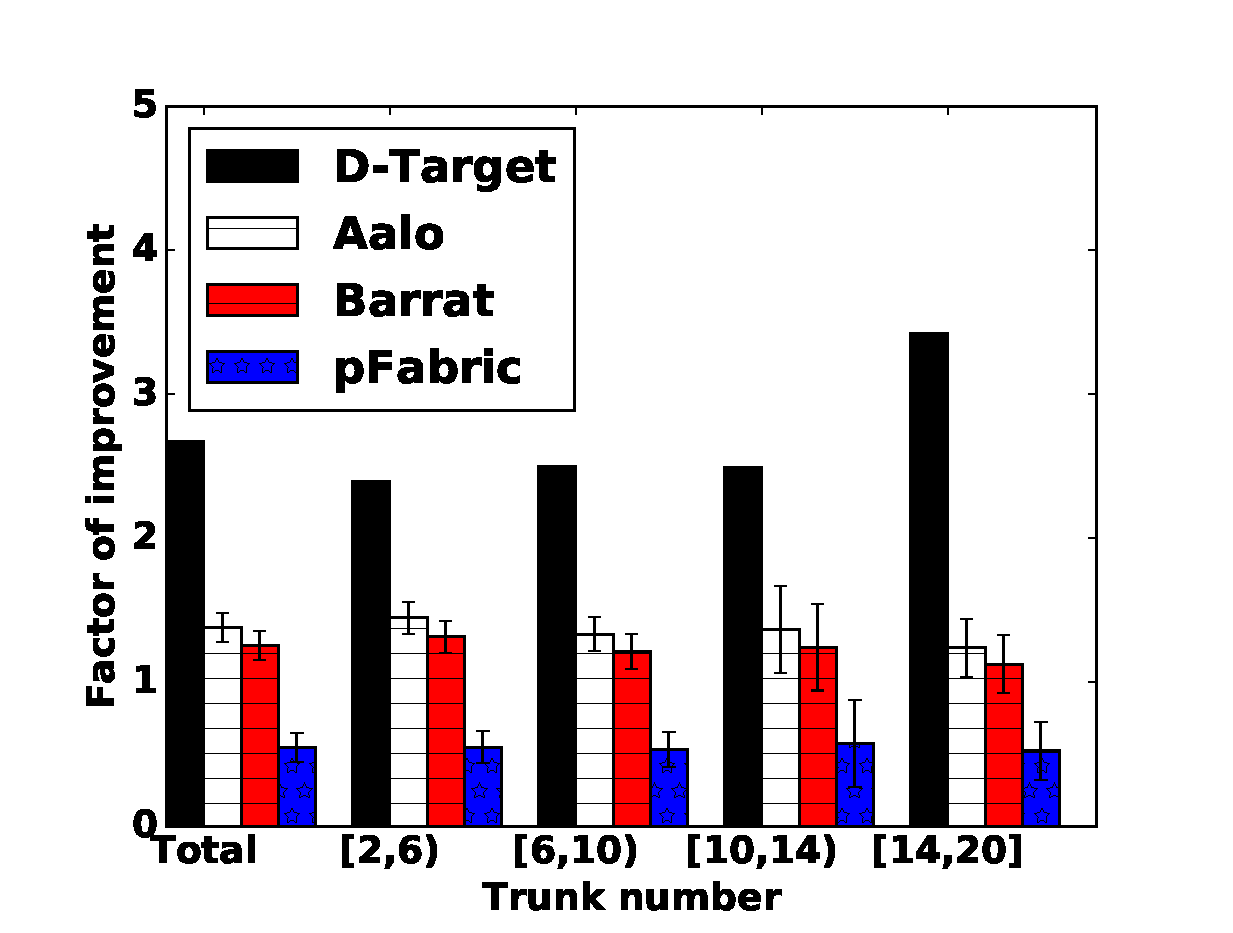
\includegraphics[width=2.1 in]{./picture/evaluation/ex1/total.eps}}
\hspace{0.1in}
\subfigure[Average FAT with SLF comparison] {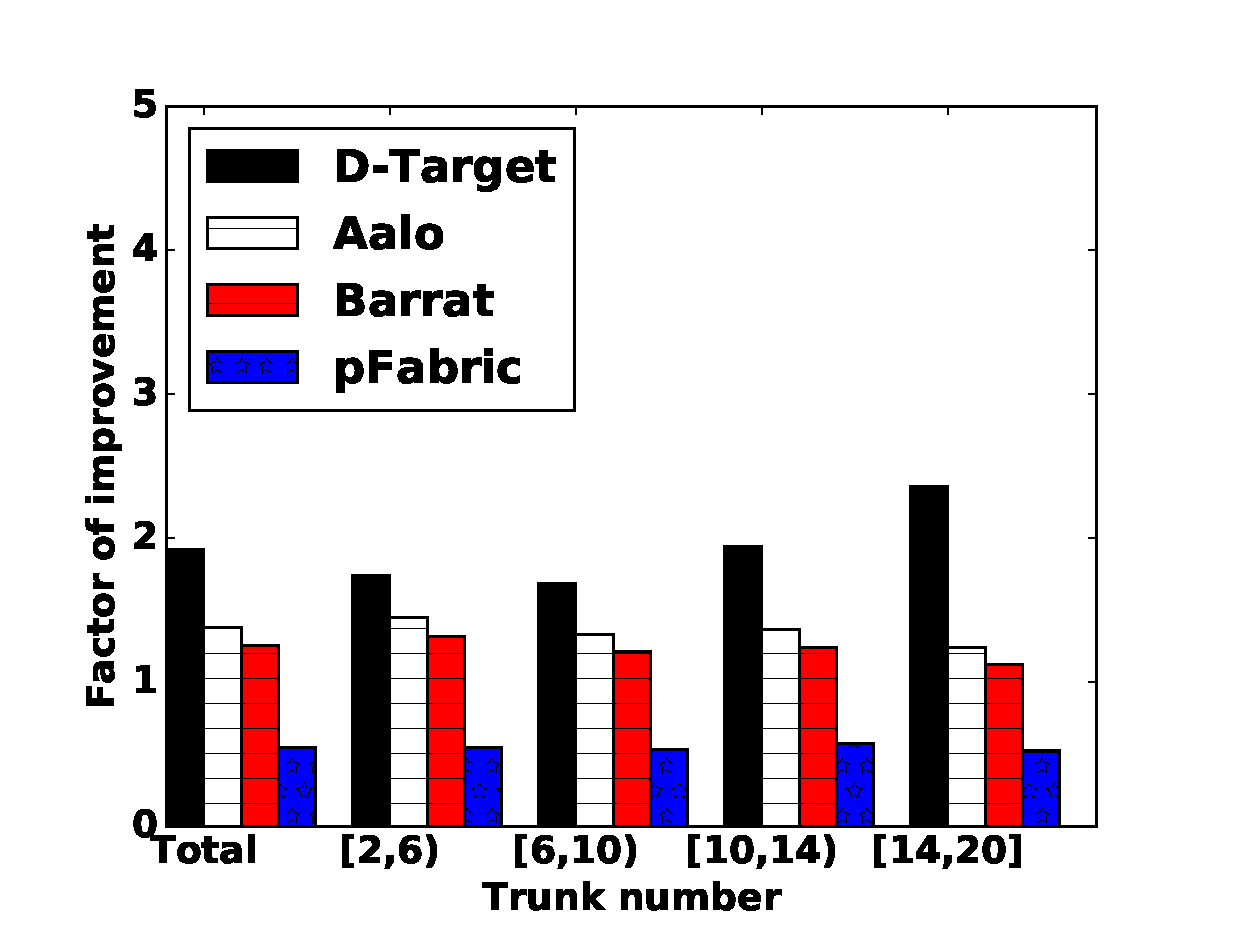
\includegraphics[width=2.1 in]{./picture/evaluation/ex1/random_select.eps}}
\hspace{0.1in}
\subfigure[With and without SLF comparison] {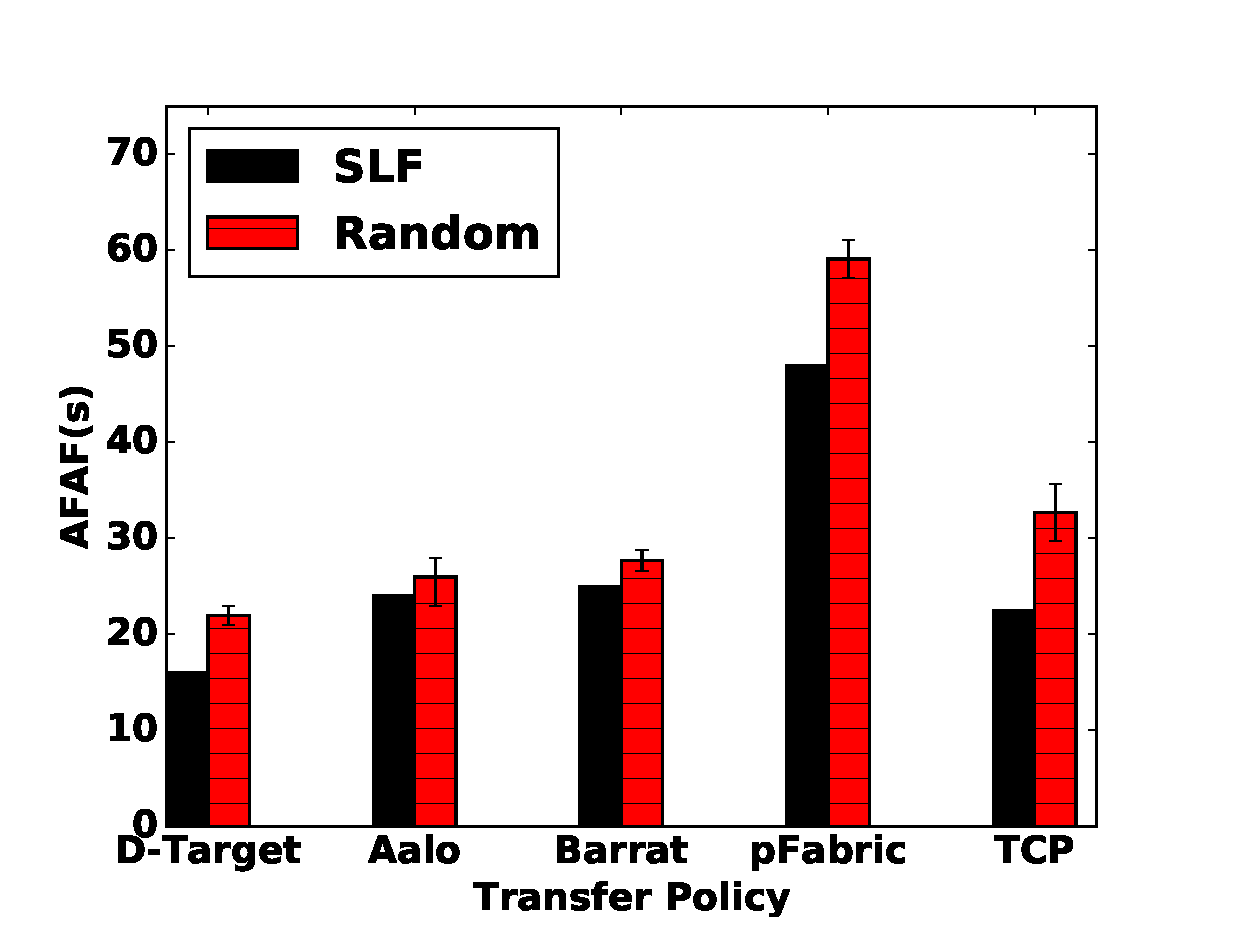
\includegraphics[width=2.1 in] {./picture/evaluation/ex1/diff.eps}}
\caption{Results with AT$\&$T trace, TCP is selected as the baseline. Note for random selection, source results are different every time, to eliminate accidental fluctuation, we run the trace 100 times for each group. }
\label{trace_fig}
\vspace{-0.1 in}
\end{figure*}


\subsection{Performance under different settings}

In this part, we explore D-Target's performance under different settings. 
We know that FAT is influenced by source selection and trunk transfer time.
For distributed erasure coding storage system, a file is encode by  $(n, k)$ MDS code,
where $n$ denotes the number of chunks that a file is encoded and $k$ denotes the number of chunks are needed to reconstruct the file.
$k$ and $n$ decides the width of the response task.
 
 
 \begin{table}[!htb]
          \centering
          \footnotesize
          \caption{Default parameters in each group of experiment} \label{tab:parameters}
          \begin{tabulary}{\textwidth}{ccccccr}
              \toprule
               Number &File size & $n$ & k & $\alpha$&Capacity&Arrival\\
              \midrule
              \multicolumn{1}{r}{512}&[100KB,10GB]   &8&4  & 1.5&1GB&[0s,1000s]\\
              \bottomrule
          \end{tabulary}
      \end{table}
      
      
      
As we want to explore the influence of each parameter, 
so in each group of experiment, we should fix the value of other parameters and only change the factor we want to study. 
TABLE \ref{tab:parameters}  shows the default settings of each experiment. 
There are 512 files and size of file is between 100KB and 10GB. 
Default parameter for MDS is value is(8,4) and the arrival time of each request is between 0 and 1000s. 
Ingress and egress port capacity in our experiment are 1GB.
 For each group of experiment, 
 we generate parameters 100 times and then draw maximum value, minimum value, average value in the picture.
 
Fig.\ref{settings_fig}(a) shows that with the increase of n, factor of improvement for D-Target becomes larger.
When n is 4, factor of improvement is 1.8 and when n is 18, factor of improvement is 2.5.
D-Target performs better for larger value of n. 
The reason for this is that for larger n, conflicts between nodes become higher, so that it is more necessary to 
optimize source selections and transfer.

Fig.\ref{settings_fig}(b) shows that with the increase of k, D-Target performs better.
When k is 3, factor of improvement is 2.2 and when k is 7, factor of improvement is 2.5, which is about 20\% larger.
For larger value of k, D-Target improves higher due to less collides.

In real word, requests can arrive at any time. 
Arrival time of requests can impact the traffic load in data center network. 
In this part, we explore the impact of transfer concurrency.  
Changing the number of requests that start at t = 0.  Fig.\ref{settings_fig}(c) shows the result. 
We can see that for larger concurrent number of requests, improvement of D-Target becomes bigger.  
This is because, the heavier the network load is, the larger optimization space there is for preemptive scheduling.


\begin{figure*}[!t]
\centering
\subfigure[Average FAT comparison] {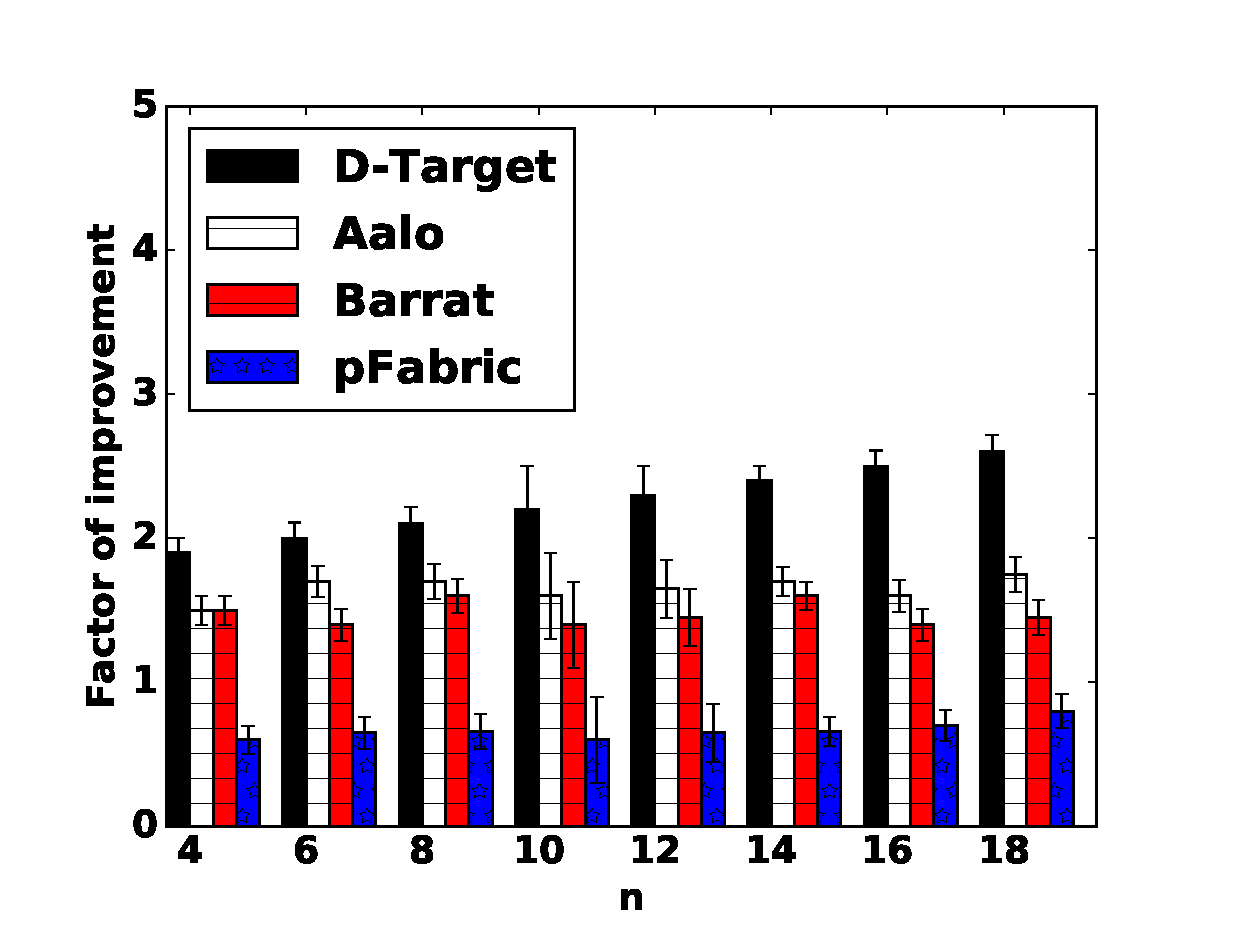
\includegraphics[width=2.1 in]{./picture/evaluation/ex2/M.eps}}
\hspace{0.1in}
\subfigure[Average FAT comparison] {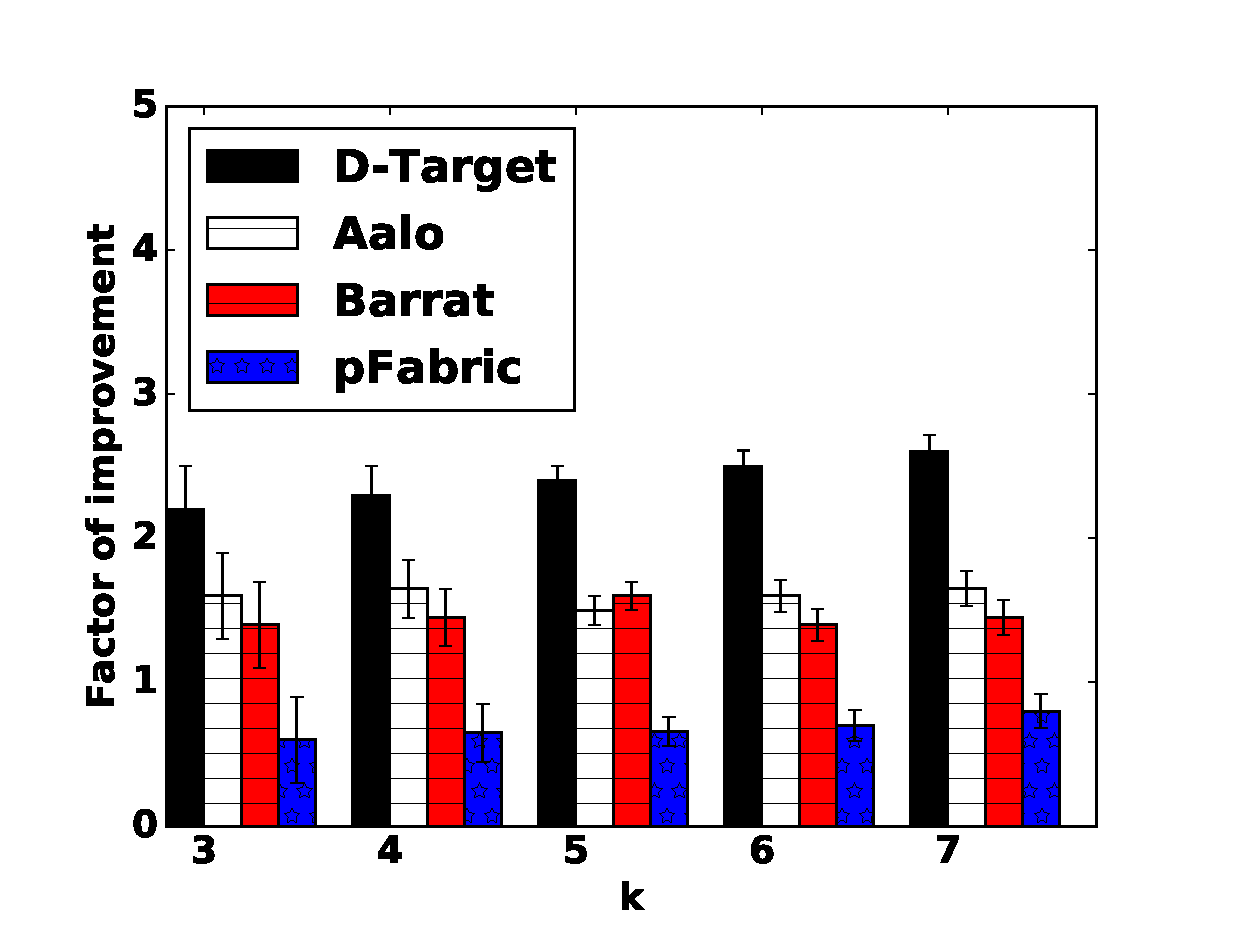
\includegraphics[width=2.1 in]{./picture/evaluation/ex2/N.eps}}
\hspace{0.1in}
\subfigure[Average FAT comparison] {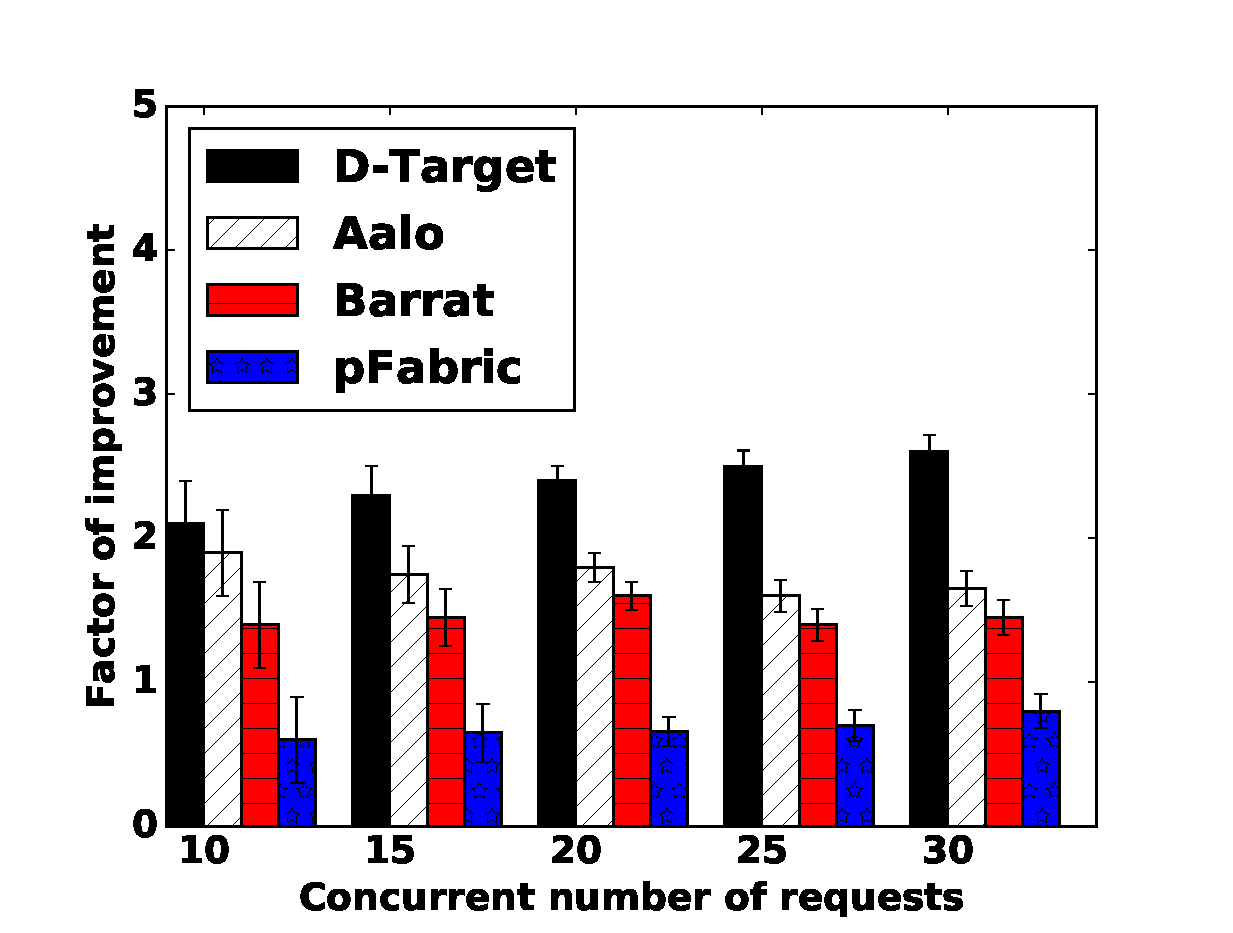
\includegraphics[width=2.1 in] {./picture/evaluation/ex2/alpha.eps}}
\caption{Performance comparison under different settings, TCP is selected as the baseline}
\label{settings_fig}
\vspace{-0.1 in}
\end{figure*}

\subsection{Distance of the online method}


Comparing with the offline 2-approximate algorithm, 
algorithm \ref{online-algorithm} ignores load diversity and this may lead to performance loss. 
In this section we study the performance gap between the online and the 2-approximate offline algorithm. 
Use the trace of AT$\&$T and set all the request arrive at t = 0, then Fig. \ref{loss_fig} shows the result.

From Fig. \ref{loss_fig}(a), we can see that factor of improvement for the 2-approximate method is 2.4, while for the online method is 2.1.
The online method has about 15\% performance loss.
Fig. \ref{loss_fig}(b) demonstrates the distribution of FAT, we can see that more than 80\% of the FAT is less than 300s for the 2-approximate method, while that for the online method is about 65\%.
Fig. \ref{loss_fig}(c) shows the performance of the two methods that are without {\em smallest load first} heuristic, we can see that performance gap between the online and 2-approximate is about 18\%. 
Fig. \ref{loss_fig}(d) shows the distribution of FAT. 
We can see that about 80\% of the FAT is within 350s, which is about 30\% worse than the method with SLF. 


\begin{figure*}[!t]
\centering
\subfigure[Average FAT comparison] {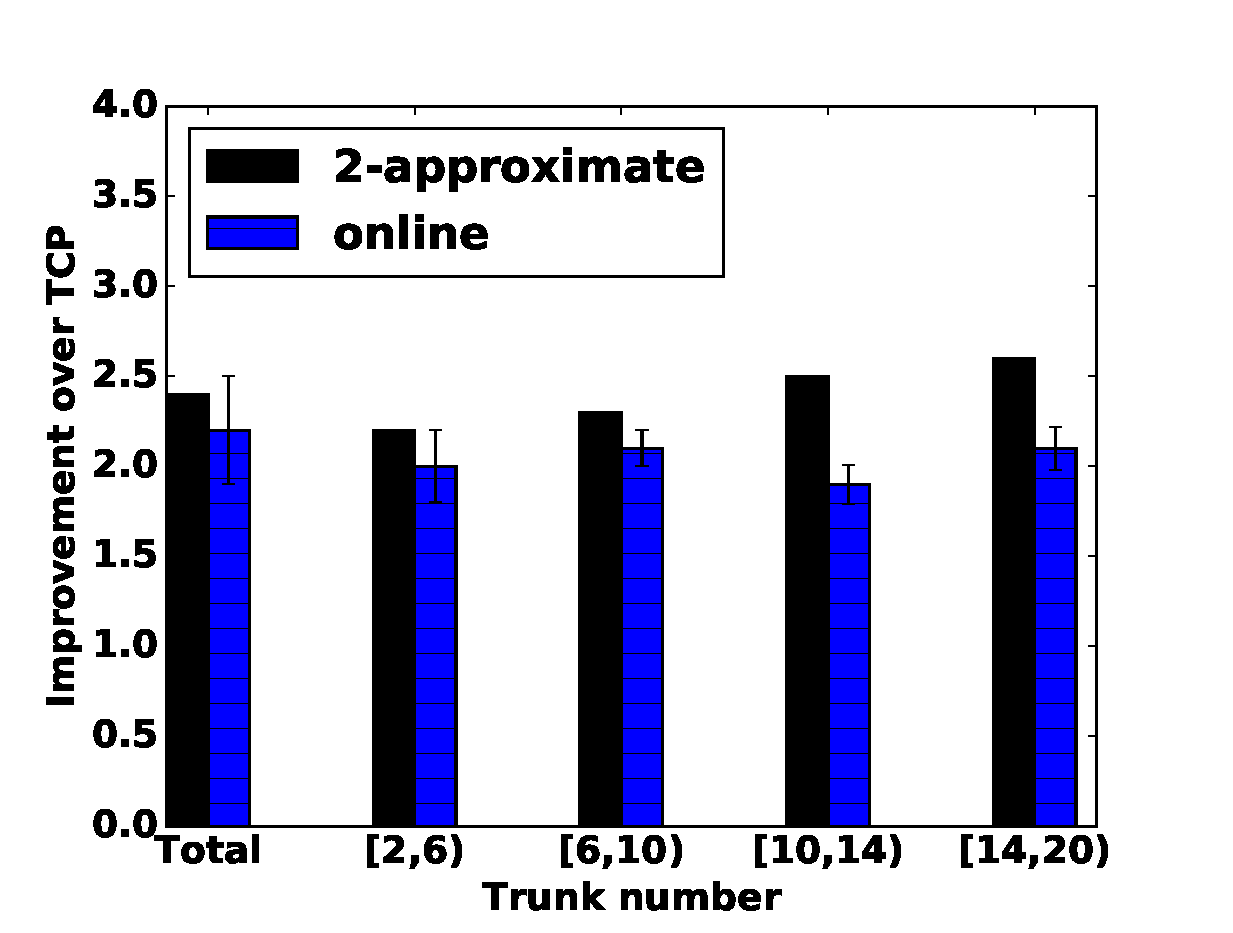
\includegraphics[width=1.5 in]{./picture/evaluation/ex3/on_off_2.eps}}
\hspace{0.1in}
\subfigure[FAT distribution] {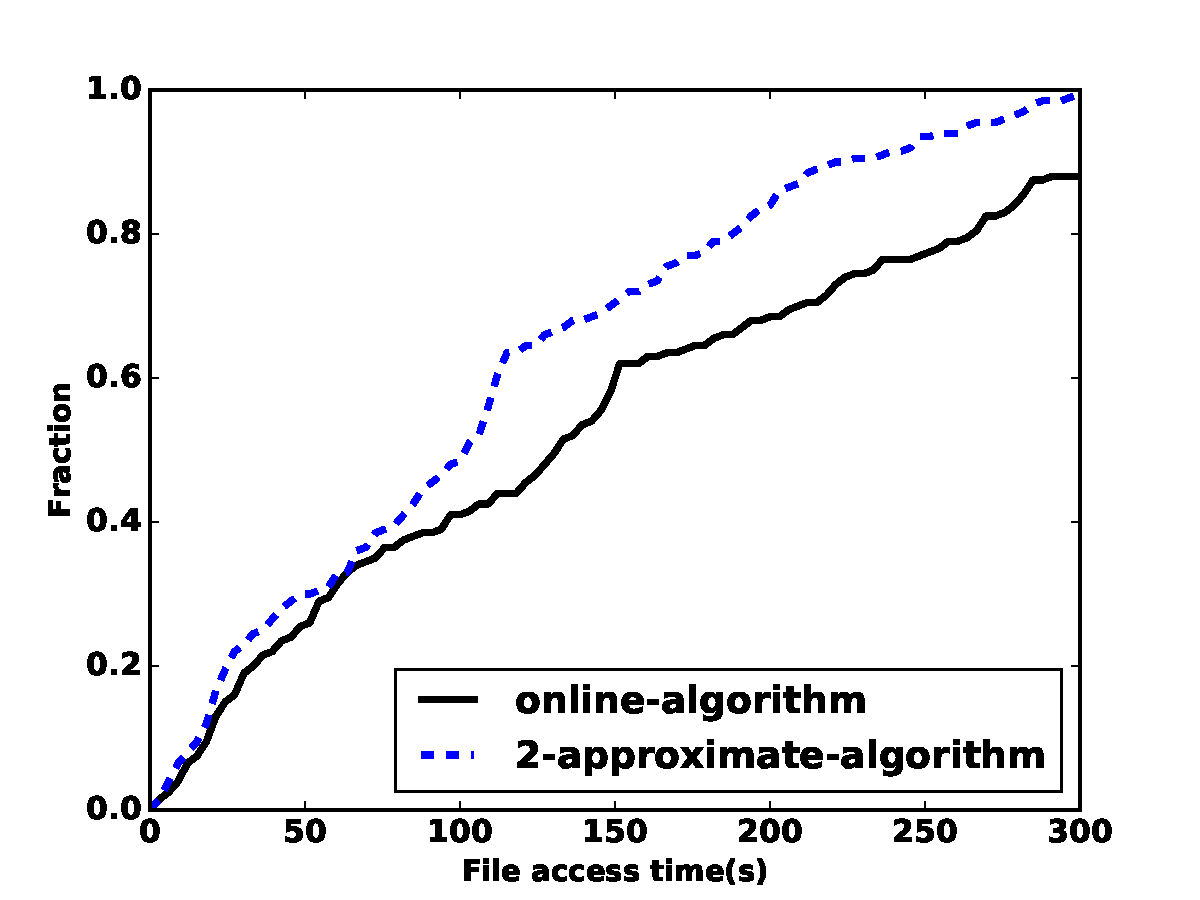
\includegraphics[width=1.5 in]{./picture/evaluation/ex3/online_offline.pdf}}
\hspace{0.1in}
\subfigure[Average FAT comparison (without SLF)] {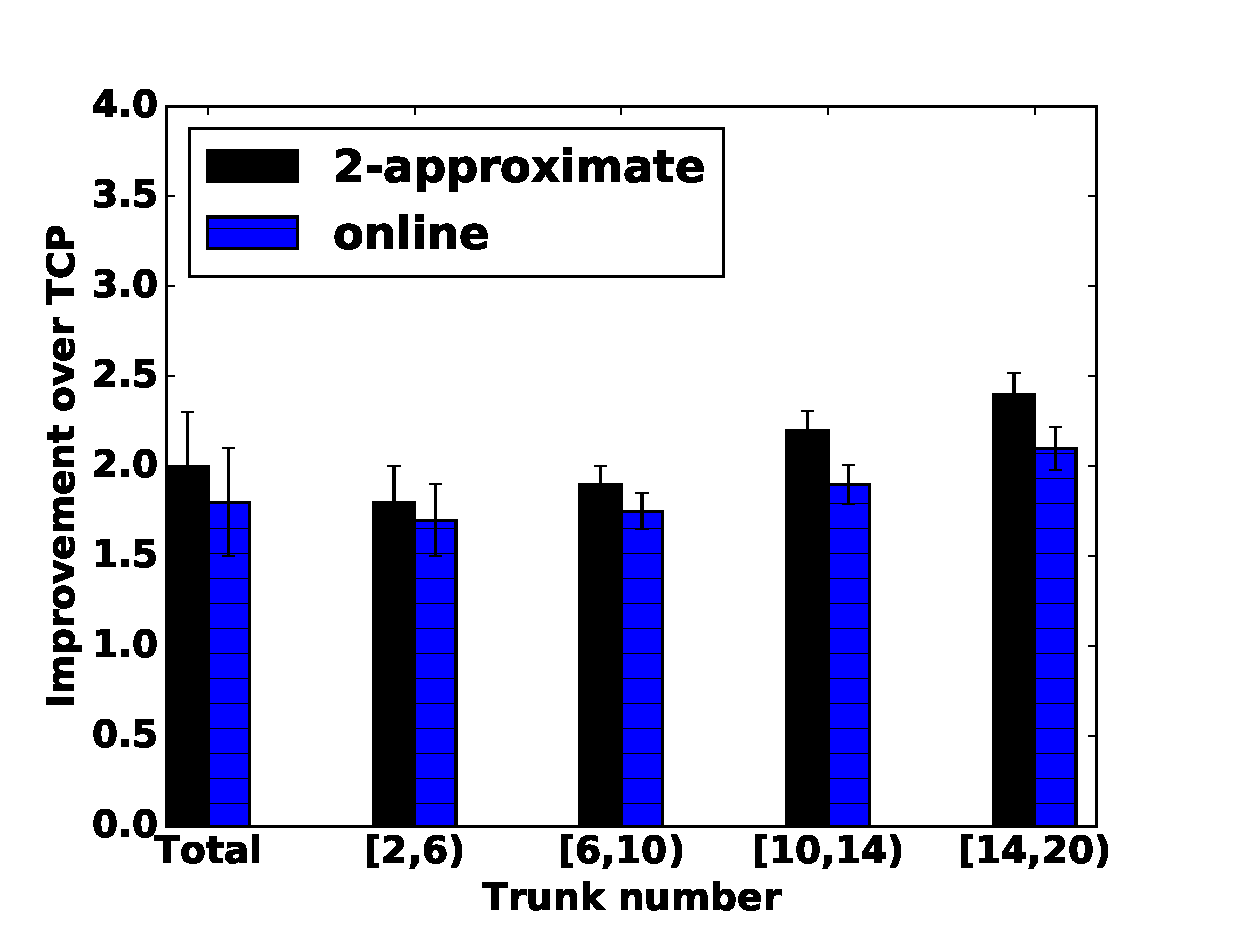
\includegraphics[width=1.5 in] {./picture/evaluation/ex3/on_off_3.eps}}
\subfigure[FAT distribution (without SLF)] {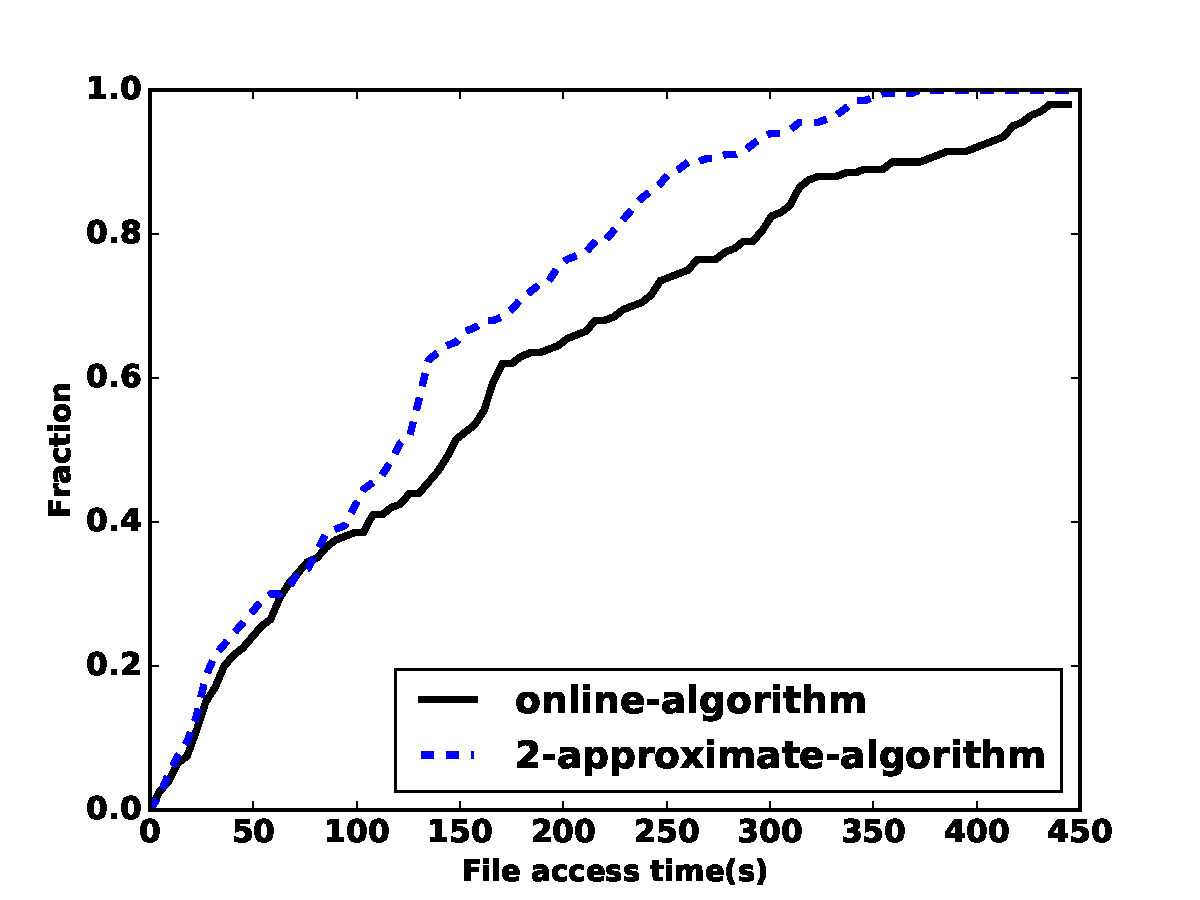
\includegraphics[width=1.5 in]{./picture/evaluation/ex3/online_offline2.pdf}}
\hspace{0.1in}
\caption{Performance comparison between 2-approximate and online algorithm. TCP is selected as the baseline.}
\label{loss_fig}
\vspace{-0.1 in}
\end{figure*}






\section{conclusion} \label{conclusion}

In this paper, we joint the two problems together to optimize.
Our optimization goal is to minimize average file access time (FAT).
To achieve this, we propose smallest load first heuristic to do source selection and design an online algorithm to reduce trunk transfer latency.
Based on this, we design and implement D-Target, a centralized scheduler that tries to minimize average FAT in distributed erasure coding storage system.
We then test D-Target's performance by trace-driven simulation.
Results show that, for the trace of AT$\&$T distribute erasure coding storage system,  D-Target performs 2.5$\times$, 1.7$\times$, 1.8$\times$, 3.6$\times$ better than TCP, Aalo, Barrat and pFabric respectively.

Now, we just test the performance of D-Target by trace-driven simulation. 
In the future, we will evaluate D-Target in the industry erasure coding storage system such as ceph \cite{Ceph
}and deploy it in real world.


\bibliographystyle{abbrv}
\bibliography{ATC}




% that's all folks
\end{document}


